\chapter{シンチレーション検出器\\(間接変換型検出器)}
\if0
臨床で用いられるCTの光センサーはフォトダイオード(PD)が現在のCTでは最も多く使われている。PDは構造が単純で小型化が容易であり、印加電圧が小さく消費電力が小さいという利点がある。しかし、素子自体が増幅機能を持たfiないため信号が小さくノイズに弱いことが最大の欠点である。そのため、鮮明なCT画像を取得するためには$10^{8-9}$cts/mm$-2$もの量のX線照射量が必要となっている。つまり「信号がノイズに埋もれない」ことが、現在のCTのX線照射量を決める要因となっていいる。\\
そこで本研究では素子の内部増幅機能に着目し、内部増幅を持つアバランシェフォトダイオード(Avalanche Photodiode: APD)、またはMulti-Pixel Photon Counter (MPPC)を利用することでノイズの影響を極端に抑え、PDを用いた従来型CTよりはるかに低線量で同等以上の画像の取得が可能であると考えた。またその低線量下であればMPPCによるフォトンカウンティングも可能となり、エネルギー情報を利用した多色イメージングも実現できCTの画像診断に新たな可能性を切り拓くことができる。本章では従来の光センサーであるPDと次世代光センサーAPDとMPPCの基本特性について述べる。
\fi
従来のX線CTの検出器にはシンチレータとフォトダイオード(Photodiode : PD)が最もよく用いられる。本章ではまずシンチレータの特徴とPDの構造と性能について述べ、その後内部増幅機能を持つアバランシェフォトダイオード(Avalanche Photodiode : APD)、Multi-Pixel Photon Counter (MPPC)それぞれの構造や性能について述べる。

\section{シンチレータ}
シンチレータとは放射線を吸収して,そのエネルギーによって蛍光する物質の総称である。シンチレータは通常,放射線を吸収したらすぐに蛍光を発し始める($10^{-8}$s 以内)。その時間変化
は以下の簡単な指数関数で近似することができる。
\begin{align}
N=\frac{N_0}{\tau_d}\exp{\left(-\frac{t}{\tau_d}\right)}
\end{align}
ここで,$N$ は時間ごとの発光した光子数で,$N_0$ は発光した光子の総数,$\tau_d$は減衰時定数である。立ち上がり時間は減衰時間よりも短く,上の式では簡略化のために省略してある。また,減衰時定数はシンチレータの種類によって固有のものである。\\
\ \ シンチレータには大きく分けて,有機シンチレータ,無機シンチレータ,プラスチックシンチレータがあるが,本節ではCTに用いられる無機シンチレータの原理と特徴を説明する(\Fref{fig:sinti})。
\begin{figure}[H]
 \begin{center}
 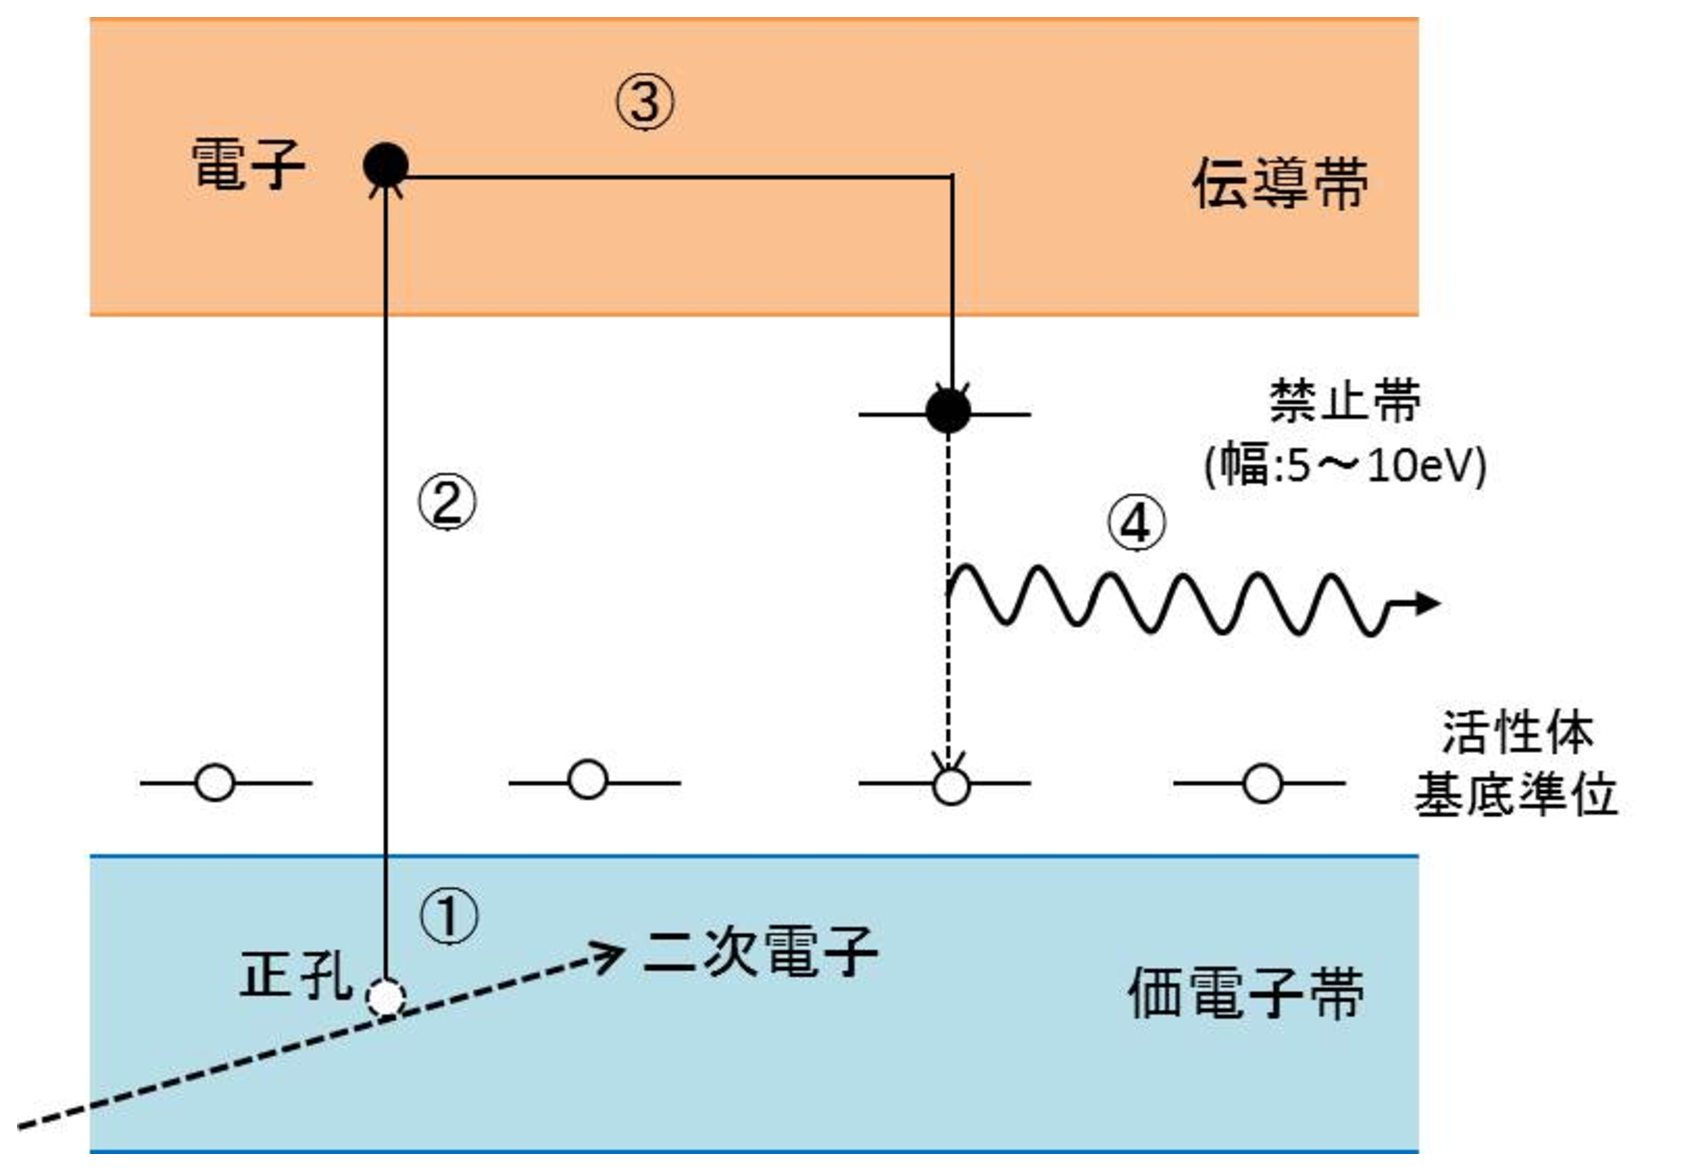
\includegraphics[width=8cm]{image/other/sinci.eps}
 \end{center}
 \caption{シンチレータの発光原理\cite{QA}}
 \label{fig:sinti}
\end{figure}

\begin{enumerate}
\item 入射光子が無機シンチレータ中に入ると前章で述べたような光電吸収,コンプトン散乱,電子対生成などの相互作用を起こし,シンチレータ内に二次電子が発生し,この電子がシンチレータの束縛電子を励起することで価電子帯から伝導帯に遷移し電子-正孔対が生じる。
\item 励起された電子と価電子帯の正孔が緩く結合する(励起子:exciton)
\item 伝導帯を移動中の電子が捕獲され,活性体原子は励起状態となる。
\item 励起準位の活性体原子は寿命(蛍光時定数)に応じて可視光を放出し基底状態に遷移する。
\end{enumerate}

\if0
まず,入射光子が無機シンチレータ中に入ると前章で述べたような光電吸収,コンプトン散乱,電子対生成などの相互作用を起こし,シンチレータ内に自由電子が発生しこの電子がシンチレータの束縛電子を励起することで価電子帯から伝導帯に遷移し電子-正孔対が生じる。このとき,伝導帯には電子が価電子帯の正孔に遷移することが可能となる。しかしながら純粋な結晶の場合,電子が伝導帯から光子を放出して価電子帯に遷移する場合,禁止帯(8eV程度)が大きいため可視光とならない。\\
\ \ そこで,少量の不純物を結晶中に添加し,純粋結晶の禁止帯中に価電子帯への電子の遷移が可能な新しいエネルギー状態を形成する。入射光子との相互作用によって生じた自由電子は,電子を価電子帯から伝導帯へ上げて数多くの電子正孔対を作る。この時,活性化物質の電離エネルギーは通常の光子位置のそれよりも小さいので小さいので正孔は素早く活性化物質の位置へ移動してそれを電離する。一方,伝導帯の電子は電離された活性化物質に移動する。この結果,活性化物質は励起状態になり上がり,基底状態に遷移する際に可視光を放出する。
\fi


入射光子のエネルギーが高いほど多くの励起子が生じ,生じる可視光の光子数が多くなり,強い蛍光となる。すなわち,シンチレータによって入射光子のエネルギーに比例する蛍光をえることができる。\\\ \ また,シンチレータの中には単結晶と多結晶(セラミック)のものがあり,単結晶においては,歩留まりが悪く,大型のものは製作が困難で高額になりやすく,大型化に限界がある。一方,多結晶は大型化が容易であるが,透明度が悪いため,光子が光検出器に届きにくという問題点があるが,近年様々なシンチレータのセラミック化が研究されている。\\\ \ シンチレータに要求される特性および性質として以下のようなものが挙げられる。以下全てを満たすシンチレータは存在しないため、目的に応じて適切なシンチレータを選ぶ必要がある。

\begin{itemize}
\item 放射線エネルギーの蛍光への変換効率(発光量)[ph/MeV]が高い\ (Tl:NaI,Tl:CsI,\\
Ce:GAGG,LaBr$_3$,LaCl$_3$など)\\
\item 放射線の阻止能が高い$\propto\rho Z^4_{eff}$ (BGO,Ce:LYSO,PWOなど) \\
高密度かつ原子番号高いほど,入射放射線と相互作用(特に光電吸収)が起きやすくなり,放射線の阻止能があがりカウントレートが増える。
\item 蛍光の減衰時定数が短い\ (Pr:LuAG,Ce:LYSO,Ce:YAP,Ce:GSOなど)\\
時定数短いとパイルアップしないため,時間分解能が高くなり高計数に対応する。言い方を変えれば高速動作が可能となる。
\item 蛍光の波長分布が,光検出器の分光感度特性に適合している。\\
蛍光の波長分布と光検出器の分光感度特性が適合していると,光子が効率よく光電子に変換されるので,高い量子効率が得られる。
\item 潮解性と自発光(内在バックグラウンド)がない\\\
潮解性がある場合,空気中に置いておくと溶けるので取扱いや保管に注意しなければならない。また,Pr:LuAG
やCe:LYSOは,$^{176}$Luが$\beta$崩壊するときに放出する線を自身で検出してしまい,それがバックグラウンドノイズとなってしまう。
\end{itemize}

\Tref{sinti}に代表的な無機シンチレータの諸性質を示す。
\begin{table}[H]
\begin{center}
\scalebox{0.8}[0.8]{
\begin{tabular}{ccccccc} \hline
シンチレータ & 発光量[ph/MeV] & 最大発光波長[nm] & 減衰時間[ns] & 密度[g/cm$^3$] & 潮解性 & ref \\\hline
Tl:NaI & 41,000 & 410 & 230 & 3.67 & 有 & \cite{sinci} \\
Tl:CsI & 66,000 & 565,420 & 800$\sim$6000 & 4.51 & わすかに有 & \cite{sinci} \\
BGO & 9,000 & 480 & 300 & 7.13 & 無 & \cite{sinci} \\
LaBr$_3$ & 63,000 & 380 & 20 & 5.29 & 有 & \cite{sinci} \\
Ce:GSO & 8,000 & 440 & 60,600 & 6.71 & 無 & \cite{sinci} \\
Ce:YSO & 10,000 & 420 & 37,82 & 4.45 & 無 & \cite{sinci} \\
Ce:LYSO & 30,000 & 420 & 40 & 7.10 & 無 & \cite{sinci} \\
Ce:YAP & 10,000 & 370 & 25 & 5.50 & 無 & \cite{sinci}\\
Ce: Pr:$\rm Gd_2O_2S$(GOS) & 50,000 & 512  & 3,000 & 7.28 &  無 & \cite{hitachi} \\
Ce:GAGG & 46,000 & 520 & 88,258 & 6.63 & 無 & \cite{sinci} \\\hline
\end{tabular}
}
\end{center}
\caption{無機シンチレータとの特性比較}
\label{sinti}
\end{table}


\if0 

\begin{table}[H]
\begin{center}
\begin{tabular}{cccccc} \hline
シンチレータ & 発光量[ph/MeV] & 最大発光波長[nm] & 減衰時間[ns] & 密度[g/cm$^3$] & 潮解性 \\\hline
Tl:NaI & 41,000 & 410 & 230 & 3.67 & 有 \\
Tl:CsI & 66,000 & 565,420 & 800\UTF{FF5E}6000 & 4.51 & わすかに有 \\
Na:CsI & 40,000 & 420 & 630 & 4.51 & 有 \\
BGO & 9,000 & 480 & 300 & 7.13 & 無 \\
CWO & 2,800 & 500 & 3, 17 & 7.90 & 無 \\
PWO & 410 & 440\UTF{FF5E}500 & 5\UTF{FF5E}15 & 8.28 & 無 \\
LaBr$_3$ & 63,000 & 380 & 20 & 5.29 & 有 \\
LaCl$_3$ & 46,000 & 350 & 25 & 3.79 & 有 \\
Ce:GSO & 8,000 & 440 & 60,600 & 6.71 & 無 \\
Ce:LYSO & 30,000 & 420 & 40 & 7.10 & 無 \\
Ce:YSO & 10,000 & 420 & 37, 82 & 4.45 & 無 \\
Ce:YAG & 8,000 & 550 & 70 & 4.57 & 無 \\
Ce:YAP & 10,000 & 370 & 25 & 5.5 & 無 \\
Ce:LSO & 27,300 & 420 & 35\UTF{FF5E}47 & 7.40 & 無 \\
Ce:GAGG & 46,000 & 520 & 88, 258 & 6.63 & 無 \\
Pr:LuAG & 20,000 & 310 & 20 & 6.73 & 無 \\\hline
\end{tabular}
\end{center}
\caption{代表的な無機シンチレータの諸特性}
\label{sinti}
\end{table}
\fi




\section{フォトダイオード(PD)\label{sec:photo}}



\begin{figure}[H]
 \begin{center}
 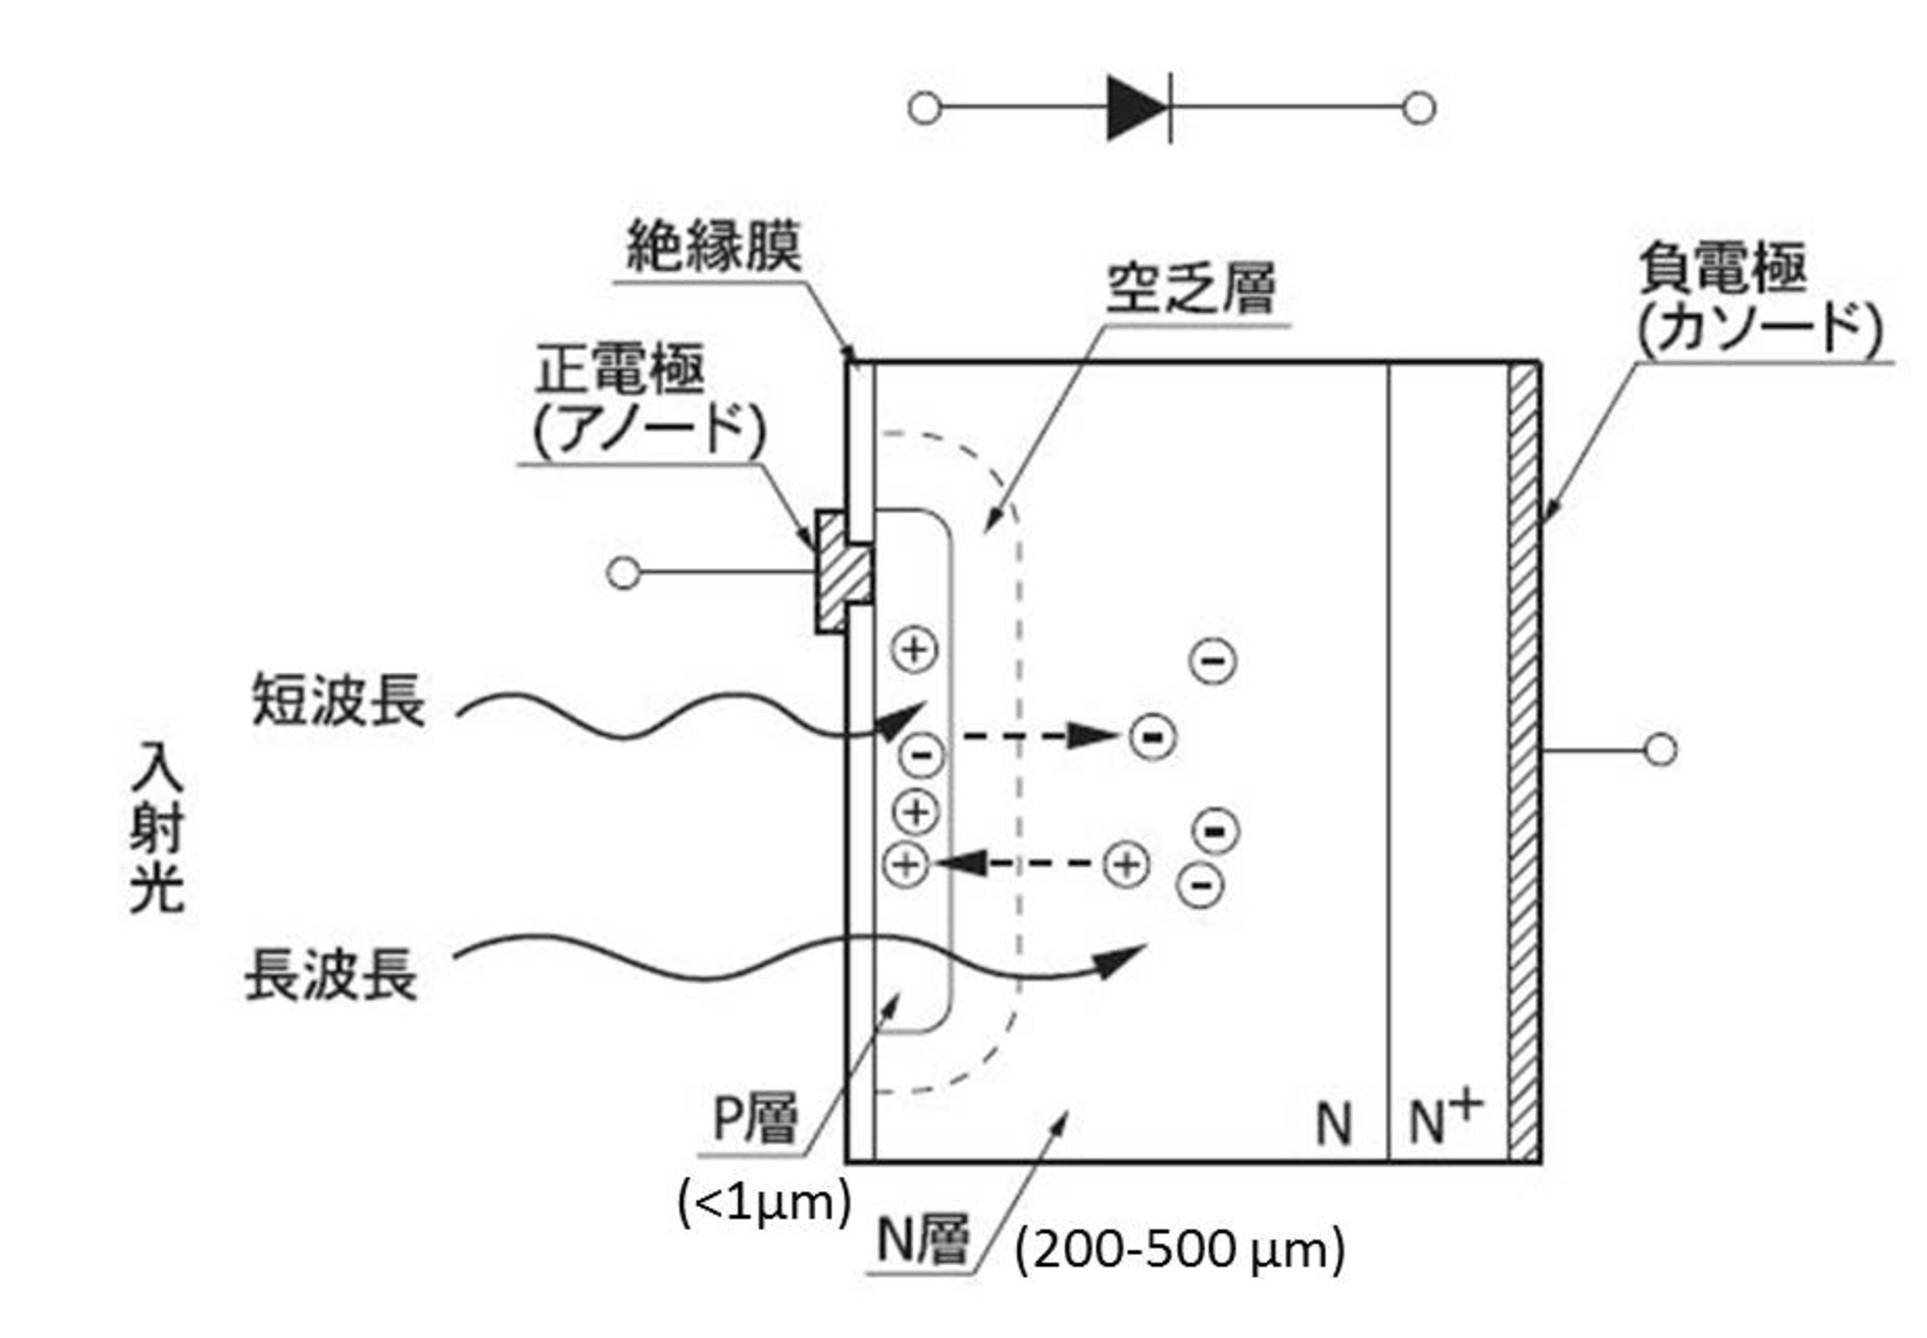
\includegraphics[width=10cm]{image/other/PIN.eps}
 \end{center}
 \caption{Siフォトダイオードの断面構造\cite{hama_hand_2}}
 \label{fig:PIN}
\end{figure}

フォトダイオード(PD)は現在のCTでは最も多く使われている光検出器である。よく用いられているPINフォトダイオードの構造を\Fref{fig:PIN}に示す。光はp型層の入射窓より入る,シリコン本体に入る光の透過をよくするため,この窓はできるだけ薄く作られている。光によって生成された電子と正孔は,逆バイアス電圧(n側が高電圧)で形成されている電界によりそれぞれの電極に収集される。ここで誘起される電荷は接続されている前置増幅器に送られ,出力パルスを発生する。\\
典型的なシンチレーション事象では可視光光子は数千個\footnote{従来のCTにはGOS(40,000ph/MeV)が用いられるが60keVがシンチレータで光電吸収されたとし、PDの量子効率を50\%とすれば生成する可視光の数は$N =60\times 40\times 0.5=1200$ 個
となる}しか生成されないのえ、得られる電荷パルスは非常に小さく、内部増幅機能も持たないためパルスモード動作ではノイズが最大の問題となる。そこで,パルスモードではなく電流モードでは頻繁に発生する多くのシンチレーション事象を蓄積することにより固有のノイズに打ち克つことが可能となり,結果的に優秀な特性を得ることができる。さらにフォトダイオードは構造が単純で小型化が容易かつ印加電圧が数十$\sim$数百Vで十分なので消費電力が少ないことから、シンチレータと組み合わせ電流モードで読み出すことで、X線CTの光検出器として選択されるようになってきた。\\
フォトダイオードの電子ノイズとして次の三つのものが最も重要である。
\begin{enumerate}
\item 並列ノイズの成分であるバルク中に生成される漏れ電流のゆらぎ
\item もう一つの並ノイズの成分である表面の漏れ電流のゆらぎ
\item 直列ノイズ源である直列抵抗に伴うノイズあるいは検出器の電気接触不良
\end{enumerate}
また、暗電流の温度依存性を\Fref{fig:PD_darkcurrents}に示す。




\begin{figure}[H]
 \begin{center}
 \includegraphics[bb=0.000000 0.000000 400.000000 503.000000,width=0.3\hsize]{image2/chapter3/PD_dark_tmp.png} 
 \end{center}
 \caption{フォトダイオードの暗電流の温度依存性}
 \label{fig:PD_darkcurrents}
\end{figure}



\begin{figure}[H]
 \begin{center}
 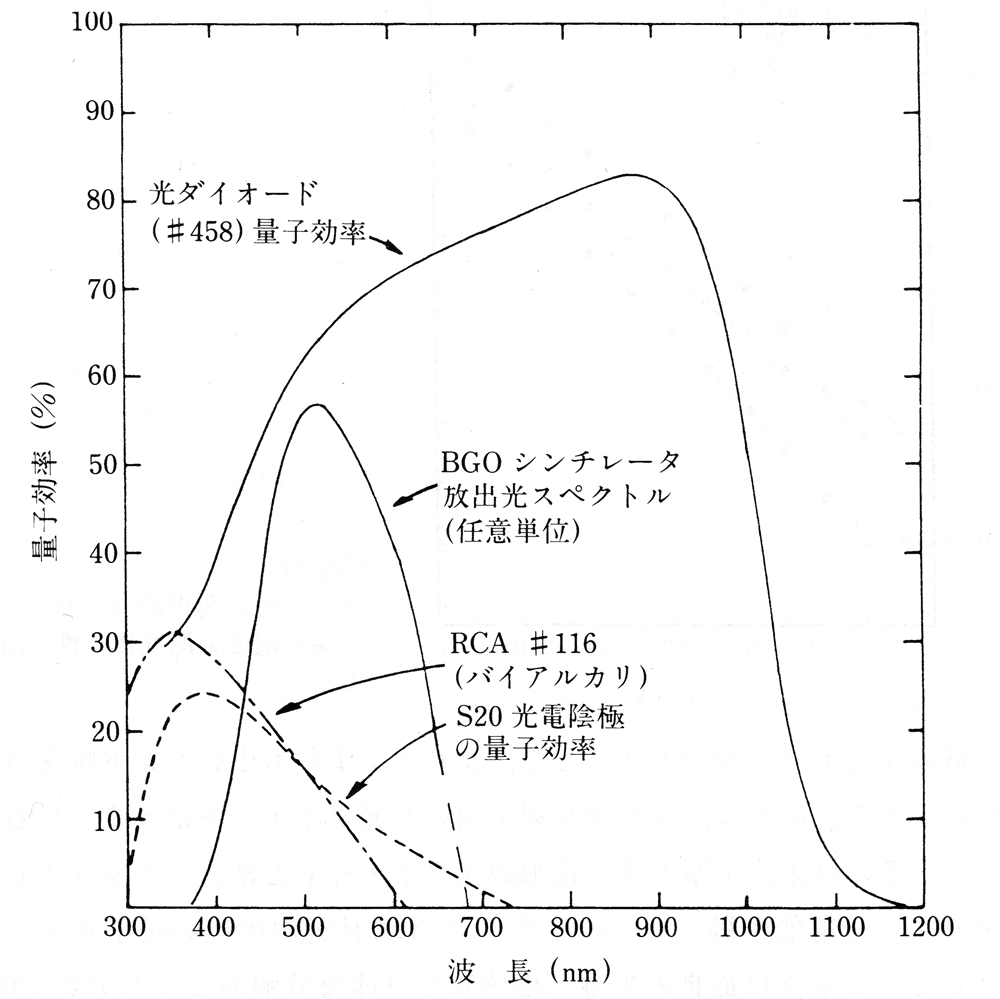
\includegraphics[width=10cm]{image/other/PD_PDE.eps}
 \end{center}
 \caption{Siフォトダイオード(#458)と代表的なバイアルカリとS-20光電面の量子効率の比較とBGOシンチレータの発光波長分布\cite{radiation_handbook}}
 \label{fig:ryousi_PD}
\end{figure}


以下にフォトダイオードのシンチレーション計数(間接型検出)における,利点・欠点についてまとめる。
\begin{itemize}
\item 利点

\begin{itemize}
\item 構造が単純で小型化が容易
\item PMTの印加電圧1000Vに対し,フォトダイオードは数十$\sim$数百Vの印加電圧で十分なので消費電力が少ない
\item 量子効率が高い(60$\sim$80$\%$)のでエネルギー分解能が高い
\item 高い量子効率が広い波長領域におよぶ
\item 磁場の影響を受けないので,磁場が存在するため光電子増倍管が使えない実験に代わりに用いることができる。
\item 電流モード読み出しにおいては安定する。
\end{itemize}

\item 欠点
\begin{itemize}
\item 増幅機能を持たないため信号が小さく,パルスモード読み出しにおいてノイズが問題となる。特に低エネルギー放射線の検出には不向きである。
\item 応答速度はシンチレータの時定数に依存する。
\item SiやGeダイオードではバンドギャップが小さいため室温おける暗電流のためノイズが多い。
\end{itemize}

\end{itemize}




\section{Avalanche Photodiode(APD)\label{sec:APD}}
PMTは高い増幅率を持つが,量子効率が低い。PDは量子効率が高いが増幅機能を持たない。PMTとPDの両方の長所を兼ね備えた光センサーがAPDである。APD においては半導体内部に高い勾配電場を作ることで,光や放射線によって電子・正孔対ができると,それが強い電場領域に入るとことで加速され,衝突電離を起こす。この衝突電離によって発生した電荷や正孔がまた同様に衝突電離を起こす,といったことを繰り返して,なだれ増幅(avalanche)を起こす。この結果,電子や正孔はM=50$\sim$100 倍まで増幅されて電極から読み出される。つまり,ノイズを等価的に1/Mに低減することで通常のPDより遥かに優れたS/N比を得ることができる。\\
\ \ APDには従来の斜めエッジ型,リバース型,リーチスルー型があるが,シンチレーション検出器としてはリバース型(\Fref{fig:reverce})が適切である。

\begin{figure}[H]
 \begin{center}
 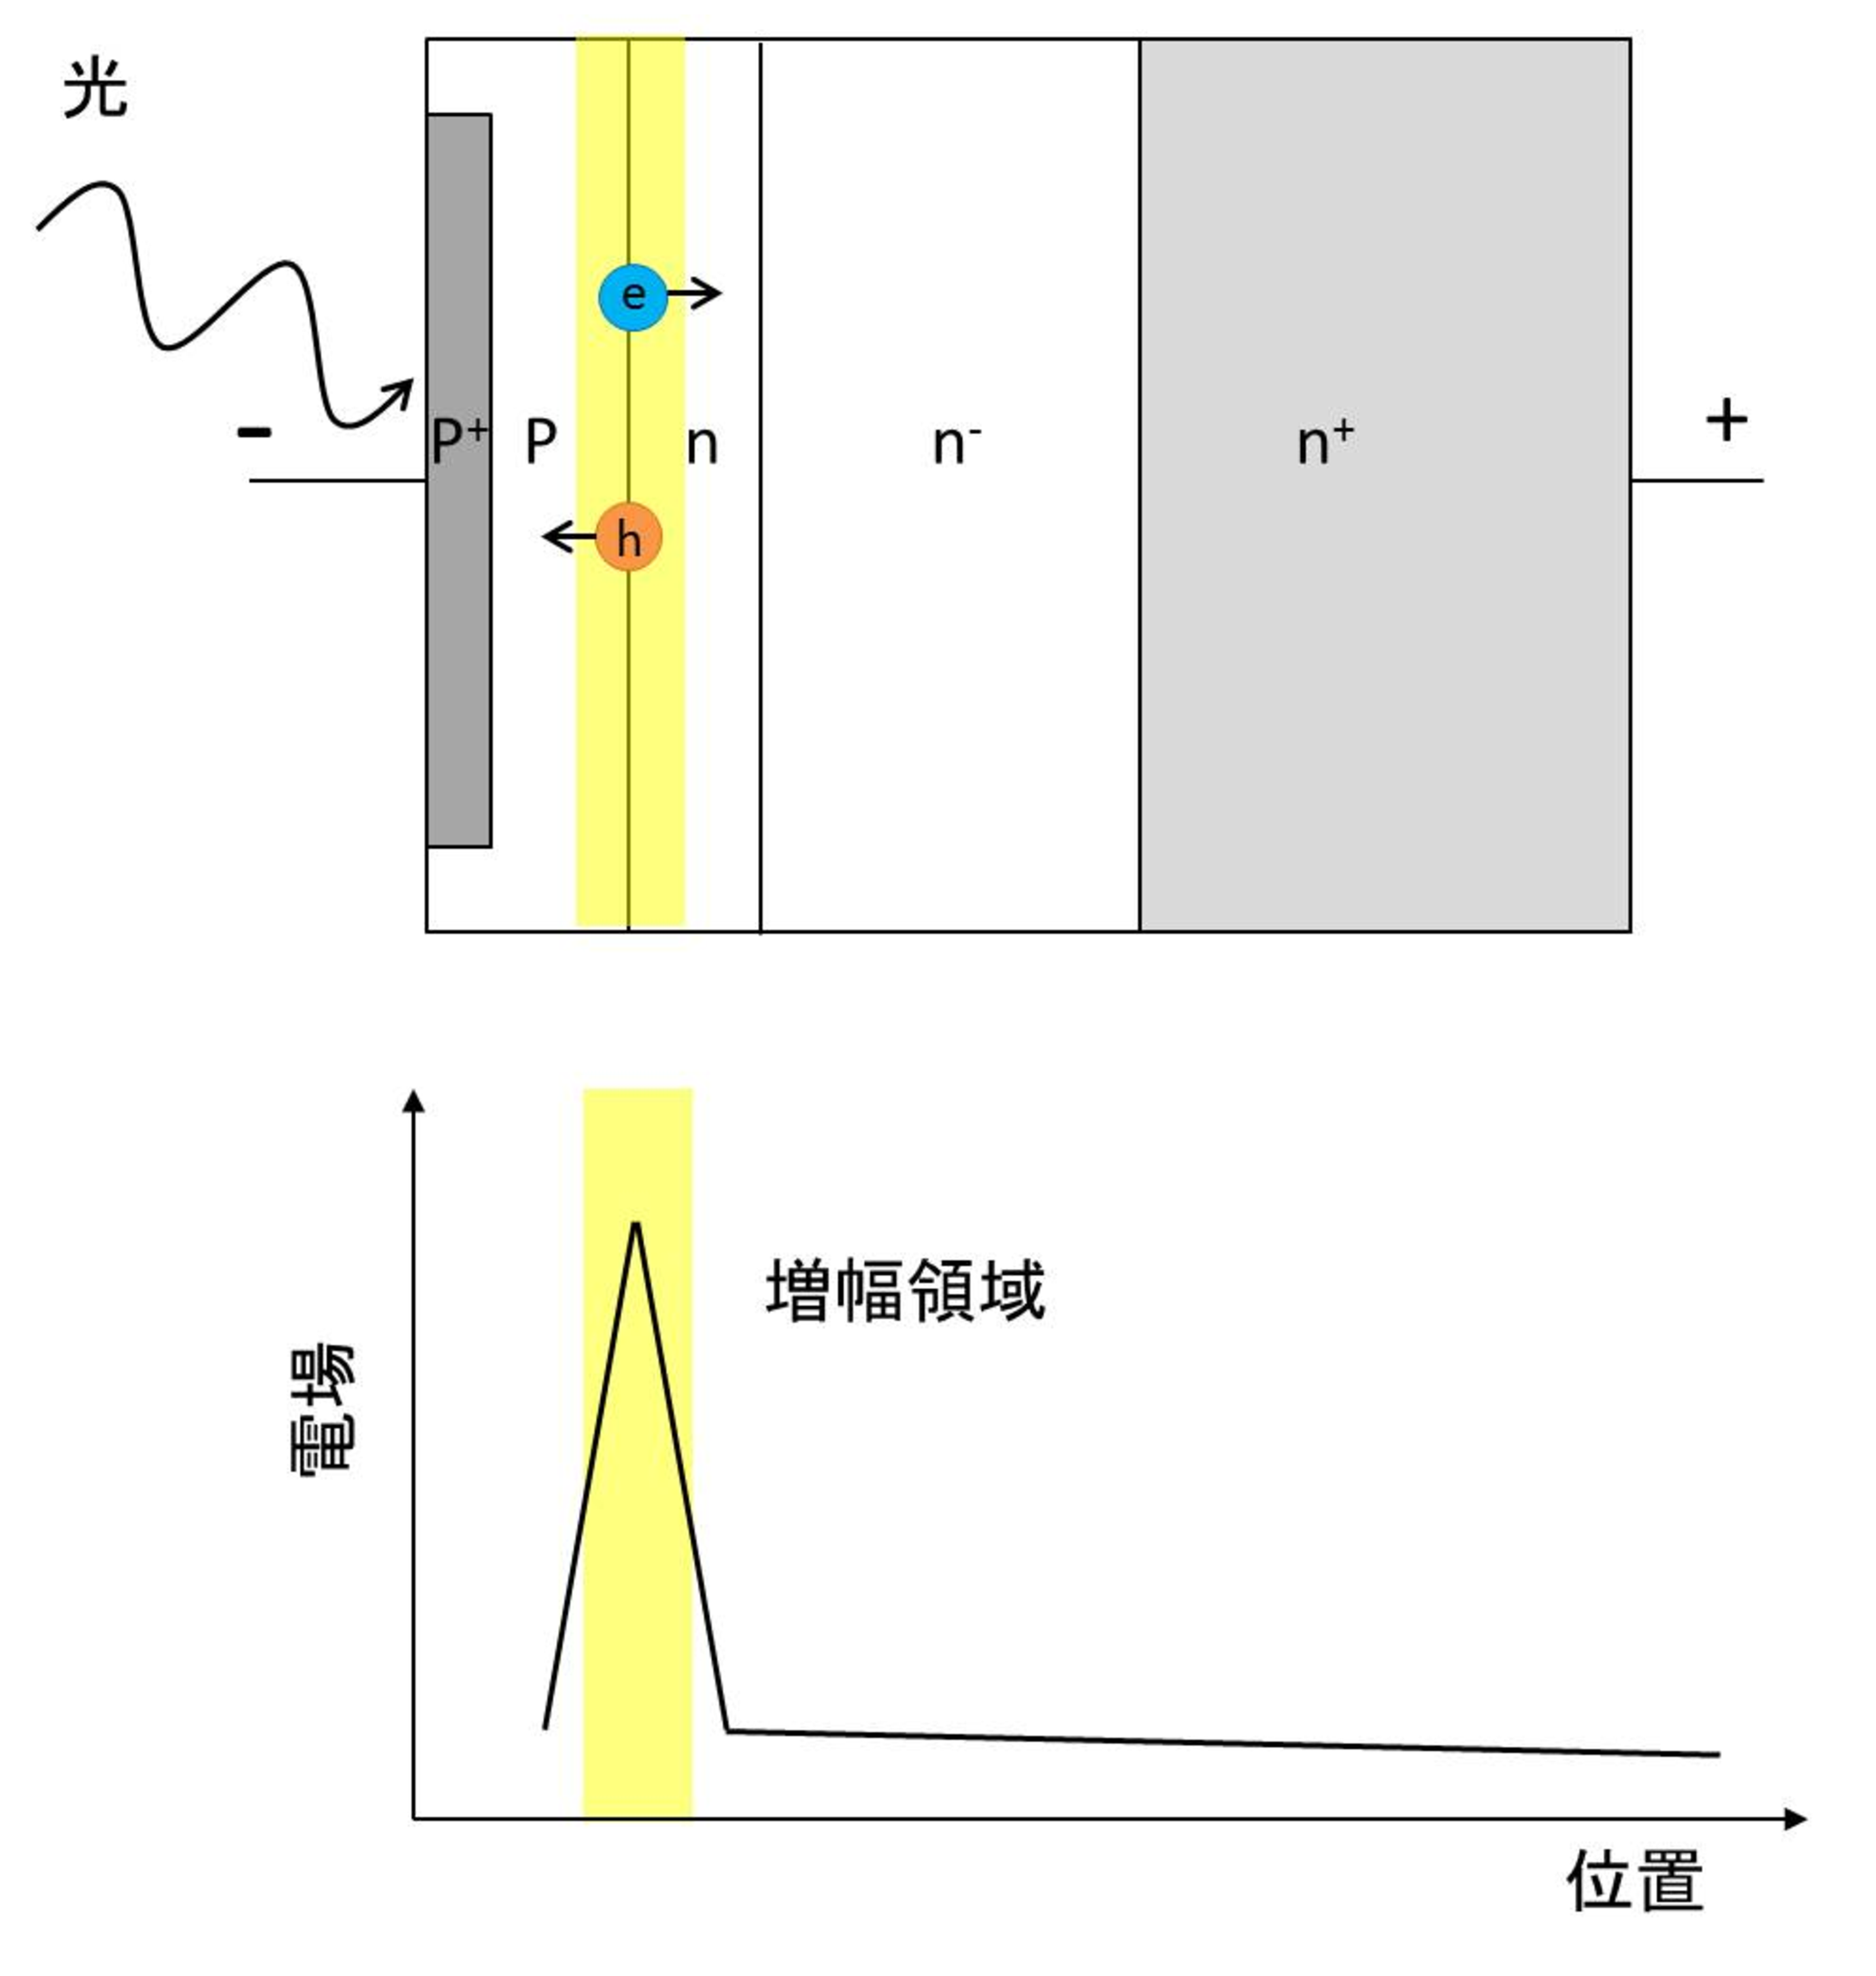
\includegraphics[width=10cm]{image/other/reverce.eps}
 \end{center}
 \caption{リバース型APDの構造\cite{kataoka_web}}
 \label{fig:reverce}
\end{figure}

この構造は入射面から$5\mu$m程度のところに増幅領域があり,シンチレーション光が表面で吸収され電子正孔対に変換されると,その全てを増幅することができる。このとき信号は増幅されるが熱電子は増幅されないので暗電流を小さくすることができノイズだけを約1/100まで低減できるのが最大の利点である。また空乏層は薄い(40$\mu$m程度)ので300-400V程度の低電圧で十分な増幅率を得ることができる。以下にAPD(リバース型)のシンチレーション検出器としての利点と欠点をまとめる。
\begin{itemize}
\item 利点
\begin{itemize}
\item PMTとPDの両者の利点(高い量子効率($\sim80\%$)\ +\ 高い増幅率(100倍))を持つので高いエネルギー分解能,高いS/N比を得る
\item 高い増幅率を得たことにより低エネルギーの放射線についてもパルスモードでの読み出しが可能となりエネルギー分解能が通常のPDより改善
\item コンパクト,低電圧動作(300-400V),磁場に強い
\item 暗電流が小さい
\end{itemize}

\item 欠点
\begin{itemize}
\item 増幅率はPMTの増幅率($10^{5-6}$)程及ばない
\end{itemize}

\end{itemize}


%一方,電流モードについては,通常のPDは増幅機能はないが固有の安定性があるのでAPDよりも好んで使われる。

\section{Muliti-Pixel Photon Counter(MPPC)\label{sec:MPPC}}
MPPCとは,Si-PM(Silicon\ Photomultiplier)と呼ばれるデバイスの一種で,個別に動作する複数のガイガーモードAPDを数十ミクロンのピッチでピクセル状に並べたデバイスである。APDの逆電圧を降伏電圧以上にするとパルス出力の大きさは入射フォトン数に関係なく素子固有の飽和出力が発生し(ガイガー放電),光子が入射したか入射しないかという情報だけが分かることになる。この電圧でAPDを動作させる状態をガイガーモードという。ガイガーモードAPDのゲインは$10^5-10^6$でありこの高い増幅率により1光子レベルの微弱な信号にも高いS/N比を実現し,微弱な光でも検出することができる。MPPCに用いられるAPDの基になっているのは\ref{sec:APD}で述べたリバース型のAPDである。MPPCの等価回路と1つのAPDピクセルと動作原理を\Fref{fig:geiger}に示す。
 \begin{figure}[H]
 \hspace{1cm}
 \begin{minipage}{0.4\hsize}
 \begin{center}
 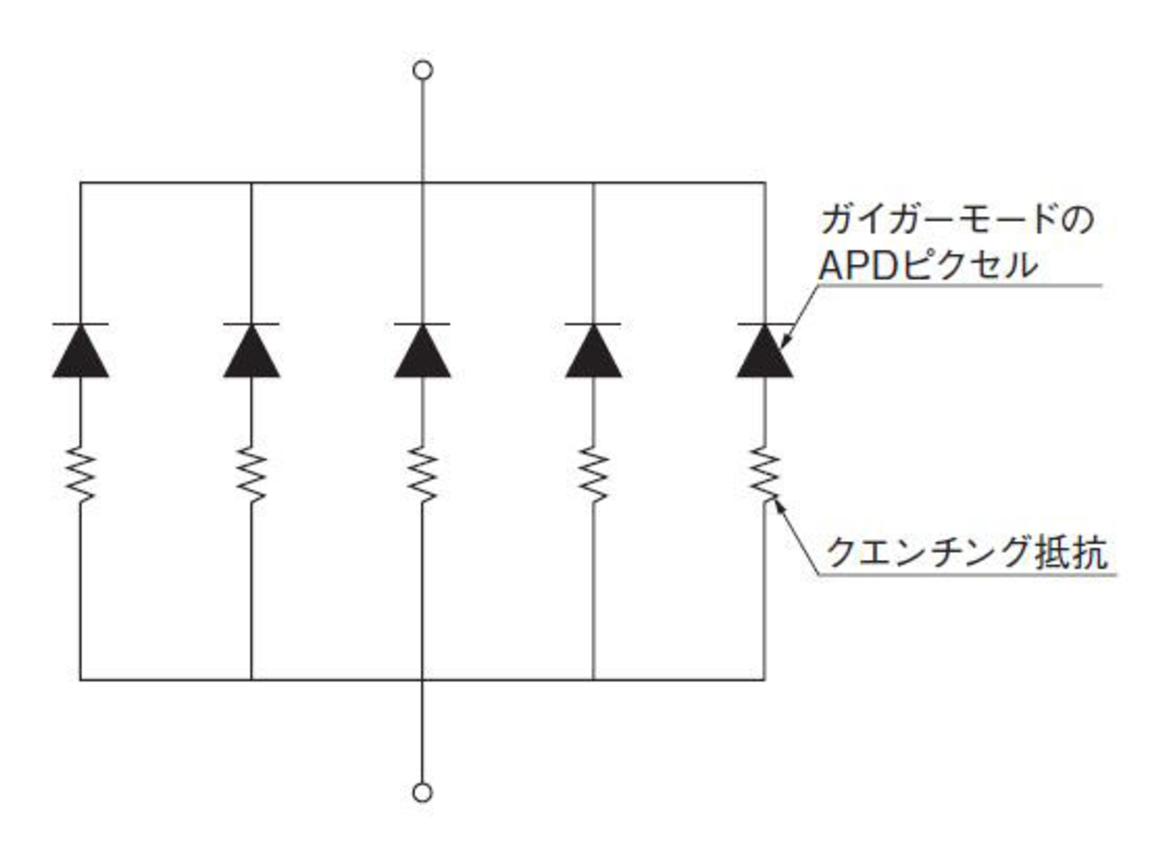
\includegraphics[width=8cm]{image/other/MPPC_touka.eps}
 \end{center}
 \end{minipage}
 \hspace{2cm}
 \begin{minipage}{0.2\hsize}
  \begin{center}
 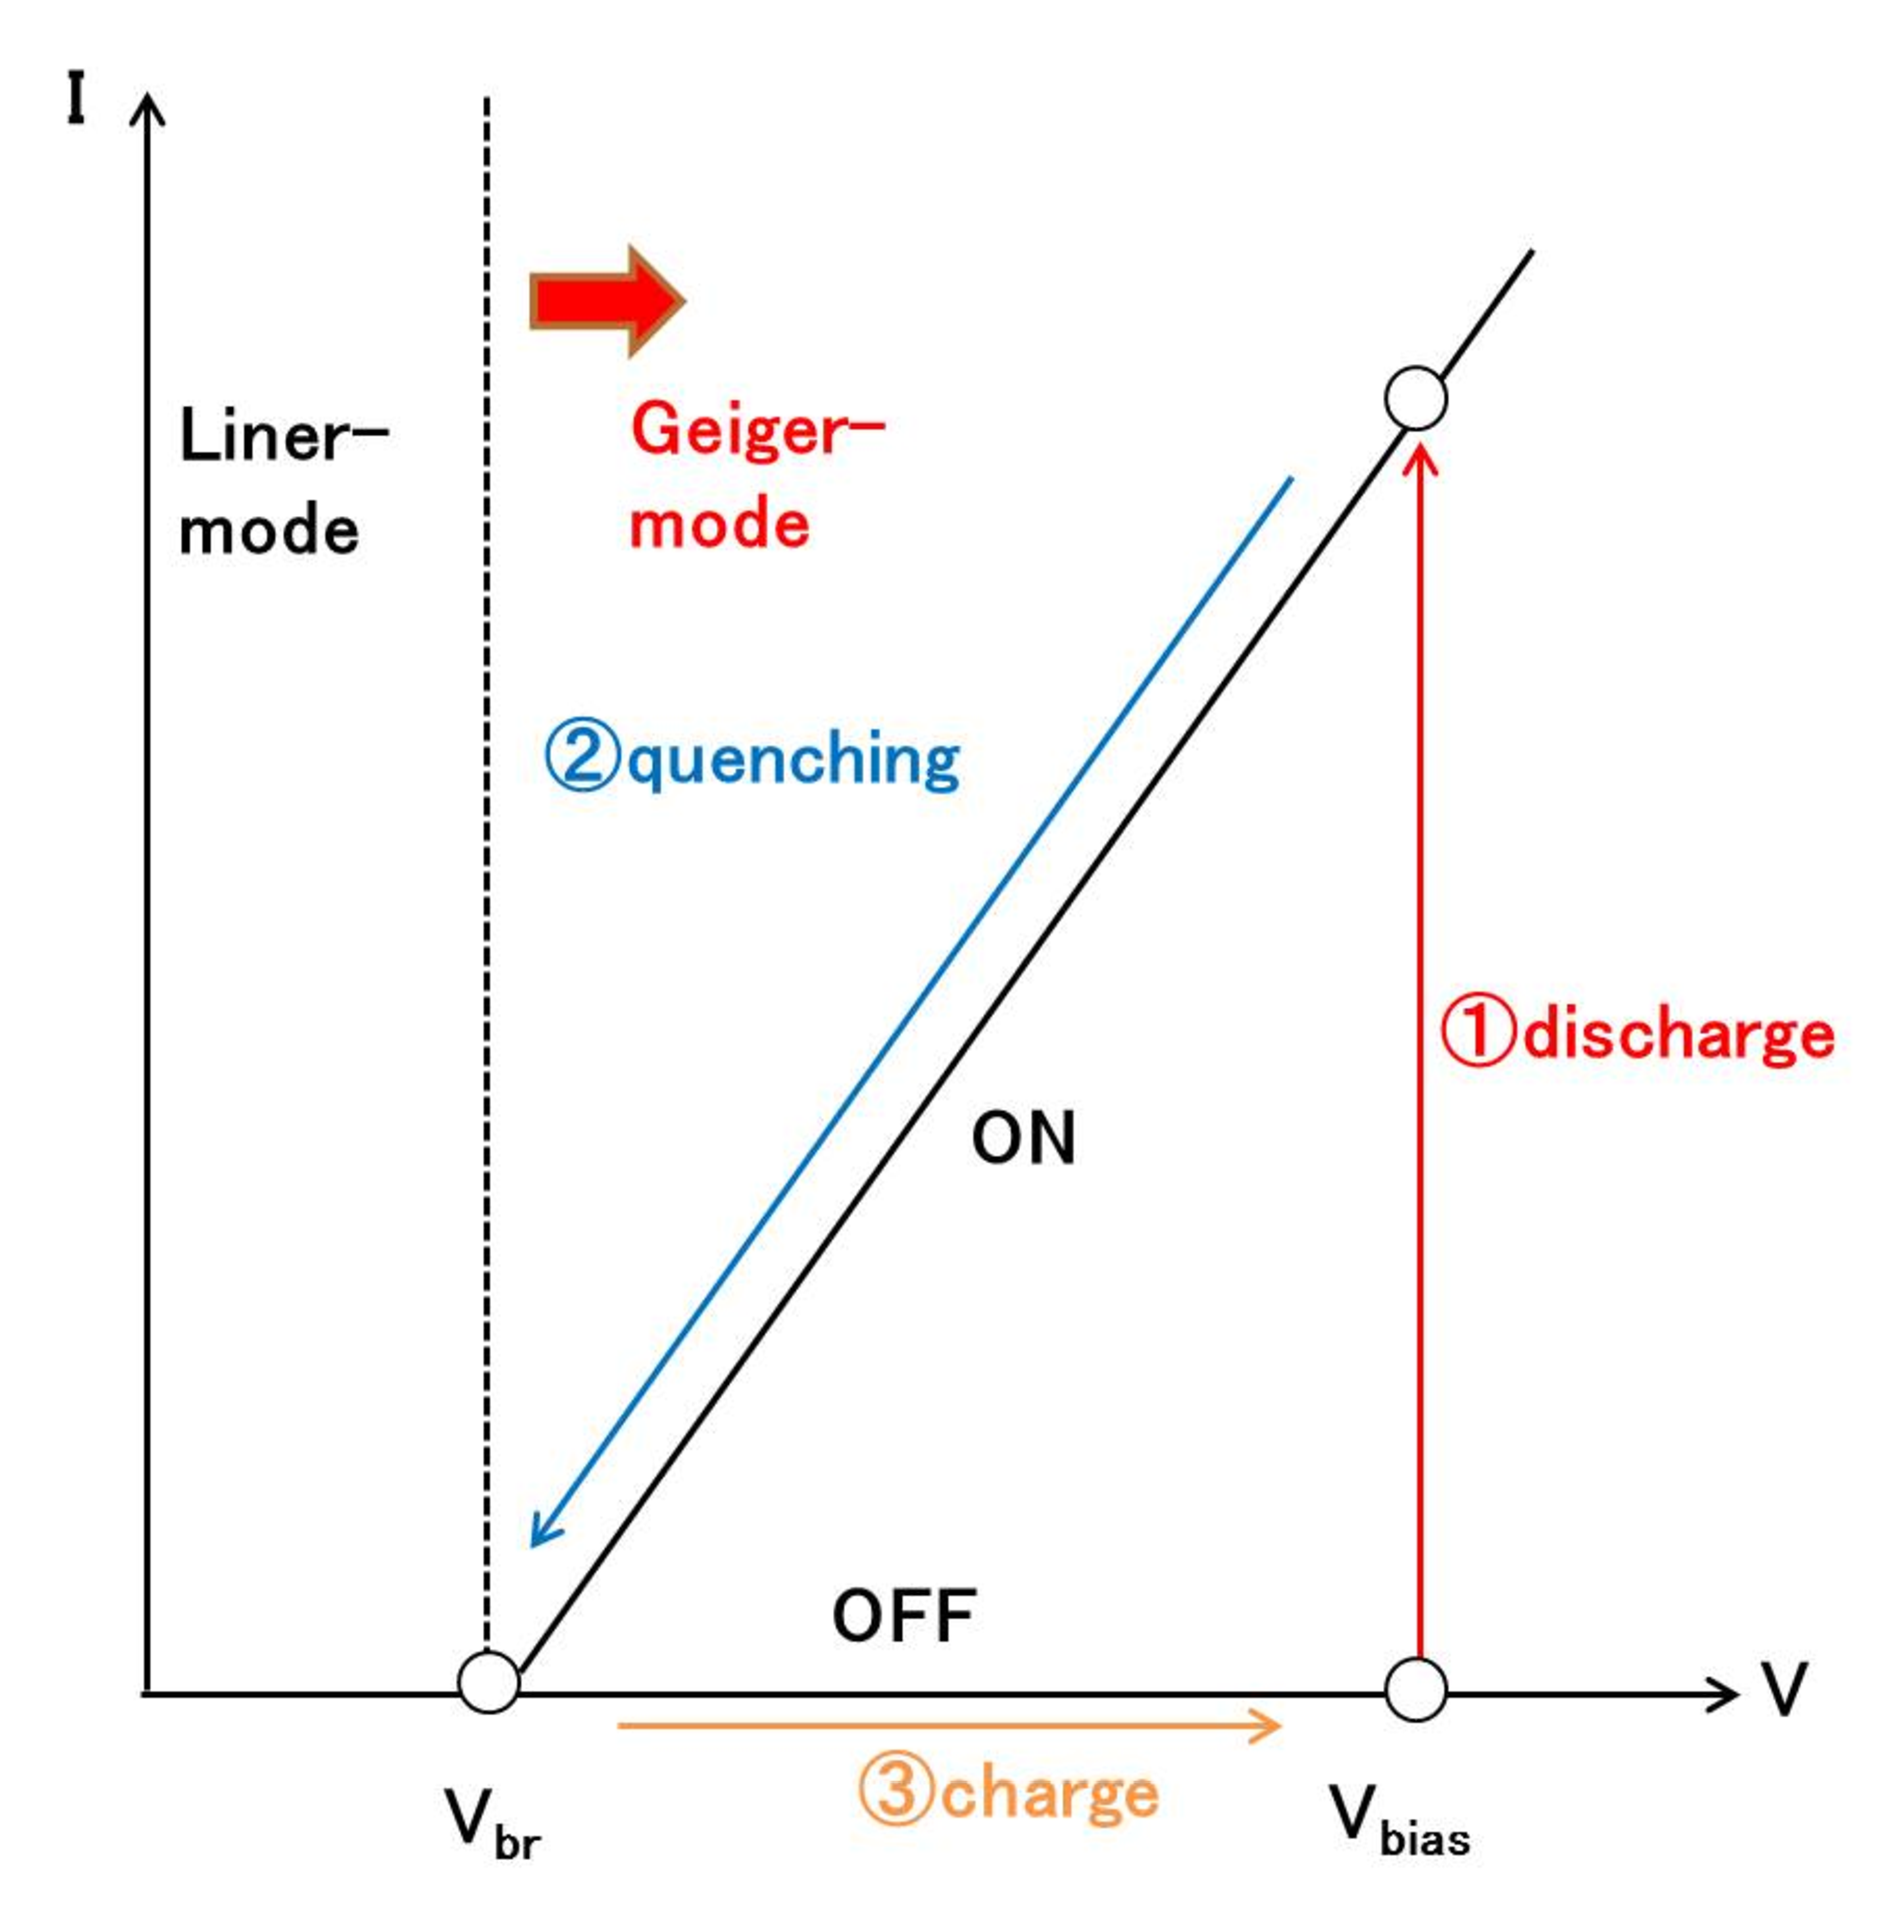
\includegraphics[width=6cm]{image/other/MPPC_cicle.eps}
 \end{center}
 \end{minipage}
 \caption{MPPCの等価回路(左)\cite{hama_MPPC}とMPPCのガイガー放電サイクル(右)}
 \label{fig:geiger}
\end{figure}

動作原理は以下の3つのサイクルの繰り返しである
\begin{enumerate}
\item 光子が入射しガイガー放電が生じる(discharge)
\item ガイガー放電された電流がクエンチング抵抗に流れると電圧降下が起こりAPDにかかる電圧が降伏電圧以下になるとガイガー放電が止む(quenching)
\item ガイガー放電が止むと電圧降下は起こらなくなり再びAPDにかかる電圧が降伏電圧以上になりガイガー放電が起きる状態となる(charge)
\end{enumerate}
この1サイクルには50ns$\sim$100nsかかりこの時間に光子が入射しても光子が検出できず不感時間となってしまう。ガイガー放電による1ピクセルからの出力電荷はAPDピクセルの容量を$C$,バイアス電圧を$V_{\rm op}$,降伏電圧を$V_{\rm br}$として以下のように書ける。
\begin{align}
Q_{\rm out}=C(V_{\rm bias}-V_{\rm br})\label{eq:out}
\end{align}
つまり,出力電荷はAPDピクセルの容量とバイアス電圧に比例する。複数のフォトンが複数のピクセルに入射するとそれぞれのピクセル出力の和がMPPCの出力となり,励起したAPDピクセルの数$N_{\rm fired}$を\Eref{eq:out}にかけた$Q_{\rm out}\times N_{\rm fired}$が全出力となる。またゲイン$M$は$M\equiv Q_{\rm out}/e$と定義されゲインもバイアス電圧とAPDの容量に比例する。APDピクセルサイズが大きい程APD容量は大きくなりゲインは上がる。またピクセルサイズが大きほどピクセルに対する受光部の割合が増え開口率があがるので検出効率が高くなる。ただしピクセルサイズが大きいほどダイナミックレンジ(同時に検出できるフォトン数)が下がる。逆にAPDピクセルサイズが小さいほど,容量は小さくないり,ゲイン,開口率,検出効率は下がるが,ダイナミックレンジは上がる。以下にMPPCの利点と欠点を示す。


\begin{itemize}
\item 利点

\begin{itemize}
\item 低電圧(100V以下)で動作可能
\item ガイガーモードで動作させることでAPDによりも高くPMTに匹敵する高いゲイン($10^5-10^6$)を持ちノイズに強い
\item 速い時間応答($\sim$100ps)
\item 小型であり磁場の影響を受けない
\item 常温でも動作可能
\end{itemize}

\item 欠点
\begin{itemize}
\item 検出効率(PDE:Photon\ Detection\ Efficiency)が高くない\\ APDよりゲインがはるかに高くなったが,クエンチング抵抗のスペース,ピクセル間がデッドスペースとなりAPDやPDほど検出効率(検出したフォトンのうち何$\%$を検出できるか)が高くない($\leq60\%$)
\item ゲインに温度依存性がある\\常温での動作が可能だがゲインに温度依存性があり,一定のバイアス電圧に対するゲインは温度が低いほど高く,温度が高いほど低くなる\footnote{温度が上がると結晶の格子振動が激しくなり,加速されたキャリアのエネルギーが十分に大きくならないうちに結晶と衝突する確率が高くなり,イオン化が起こりにくくなる。その結果温度が高いほどゲインが低くなる。}。

\begin{figure}[H]
 \begin{center}
  \includegraphics[bb=0.000000 0.000000 801.000000 692.000000,width=0.9\hsize]{image2/chapter5/MPPC_tmp.png} 
 \end{center}
 \caption{MPPCのゲインの温度依存性}
 \label{fig:MPPC_tmp}
\end{figure}


そのため一定の出力を得るには温度によってバイアス電圧を変化させるか,素子の温度を一定に保つ必要がある。
\item 入射フォトン数が多くなると励起ピクセル数と入射フォトン数の線形性が崩れる\\MPPCの全ピクセル数$ N_{\rm total}$がダイナミックレンジを決定し,全ピクセル数に対して入射フォトン数$ N_{\rm photon}$が多くなると,1ピクセルに2個以上の光子が入り始め,入射フォトン数と励起ピクセル数$ N_{\rm fired}$の線形性が崩れる\footnote{$ N_{\rm fired}= N_{\rm total}\left[1-\exp{\left(-\frac{ N_{\rm photon}\times \rm PDE}{ N_{\rm total}}\right)}\right]$}。
\item ダークカウントが生じる\\光により生成したキャリアだけでなく熱的に発生したキャリアによっても電流が発生する(ダークカウント)。これは温度が低いほど小さくなる。
\item アフターパルスが生じる\\ 発生したキャリアが結晶欠陥にトラップされ,それが遅れて解放されたときに信号以外のパルスを発生させてしまう(アフターパルス)。温度が低いほどキャリアが欠陥にトラップされる確率が高くなり,アフターパルスは増加する。
\item クロストークが生じる\\
ガイガー放電中に電子と正孔が再結合して光子が放出され,その光子をとなりのピクセルが検出してガイガー放電を起こしてしまうことがある(クロストーク)

\end{itemize}

\end{itemize}

\section{光検出器の性能比較}

\begin{table}[H]
\begin{center}
\begin{tabular}{ccccc} \hline
 & PMT & PD & APD & MPPC \\\hline
増幅率(ゲイン) & $10^{5-6}$ & 1 & 10-100 & $10^{5-6}$ \\
量子効率(検出効率) & $\leq25\%$ & \multicolumn{2}{c}{$\leq80\%$} & $\leq60\%$ \\
体積・サイズ& ×(大きい) & \multicolumn{3}{c}{$\circ$(小さい)} \\
磁場耐性 & ×(不可) & \multicolumn{3}{c}{$\circ$(可能)} \\
構造 & ×(複雑) & \multicolumn{3}{c}{$\circ$(単純)} \\
動作電圧[V] & $\thicksim1000$ & $\thicksim30$ & $\thicksim300$& $\thicksim70$ \\
電力&×(大)&\multicolumn{3}{c}{$\circ$(小)}\\\hline
\end{tabular}
\end{center}
\caption{光検出器の性能比較\cite{kataoka}}
\label{detectors}
\end{table}
それぞれの光検出器の性能比較を\Tref{detectors}に示す。どれも一長一短であり,用途により選択が必要となる。高いエネルギー分解能を求める場合,量子効率が高いPDやAPDを用いるべきであるが,この二つはゲインが低いので微弱な光つまり,低エネルギーの検出は苦手とする。微弱な光の検出をする場合高いゲインを持つPMTやMPPCを用いるべきである。\\
\ \ CTの光検出器としは小型化が可能なPDが主流である。PDを電流モードで読み出すことによりノイズに打ち勝ち低エネルギーの検出も可能としてる。しかし,フォトンカウンティングCTにおける検出器のためにはパルス読み出しを行う必要があるため高いS/N比を得ることができ,エネルギー分解能も高く,小型化が可能な検出器が求められる。

\chapter{半導体検出器(直接変換型検出)}
近年フォトンカウンティングCTの検出器として、直接検出型のCdTe,CZTなどの原子番号が高い半導体検出が用いられている。本章ではCdTeの構造とその特徴について述べる。
\section{CdTe半導体の特性}
従来,X 線やガンマ線の検出のための半導体検出器として,主にシリコン(Si)やゲルマニウム(Ge)が使用されてきた。しかし,Siは原子番号が14と低いためX線やガンマ線に対する検出効率が低く,直接型の半導体検出器としては用いることができない。Geは原子番号が32であり,検出効率は低くはなく,直接型の半導体検出器として用いることで極めて高いエネルギー分解能を得ることできる。しかしGeは室温ではバンドギャップが小さく比抵抗極めて小さいため,液体窒素温度で動作させる必要がある。そこでSi,Geよりも原子番号が高く,検出効率の高いかつ室温動作が可能な化合物半導体としてCdTe(テルル化カドミウム)やCd$_{1-x}$Zn$_x$Te(CZT)がある。それぞれの半導体の特性を\Fref{semi_chara}に示す。
\begin{table}[H]
\begin{center}
\begin{tabular}{ccccc} \hline
半導体(温度[K]) & Si(300) & Ge(77) & CdTe(300) & $\rm Cd_{0.8}Zn_{0.2}Te$(300) \\\hline
原子番号 & 14 & 32 & 48/52 & 48/30/52 \\
密度[g/cm$^3$] & 2.33 & 5.32 & 5.85 & 6.0 \\
バンドギャップ[eV] & 1.12 & 0.74 & 1.5 & 1.6 \\
電離エネルギー[eV] & 3.61 & 2.98 & 4.43 & 5.0 \\
比抵抗[$\Omega\cdot$cm] & $10^3$ & $10^2$ & $10^9$ & 3$\times10^{10}$\cite{takahashi} \\
移動度$\mu_e$[cm$^2$/Vs] & 1350 & 3.6$\times10^4$ & 1100 & 1350 \\
移動度$\mu_h$[cm$^2$/Vs] & 480 & 4.2$\times10^4$ & 100 & 120 \\
寿命$\mu_e$[s] & 2$\times10^{-5}$ & 2$\times10^{-5}$ & 3$\times10^{-6}$ & $\times10^{-6}$ \\
寿命$\mu_h$[s] & 2$\times10^{-5}$ & 2$\times10^{-5}$ & 2$\times10^{-6}$ & 2$\times10^{-7}$ \\
$\mu_e\tau_e\rm[cm^2/V]$ & 0.42 & 0.72 & 3.3$\times10^{-3}$ & $\sim10^{-3}$ \\
$\mu_h\tau_h\rm[cm^2/V]$ & 0.22 & 0.84 & 2$\times10^{-4}$ & $\sim2\times10^{-5}$ \\
参考文献 & \cite{sakai} & \cite{sakai} & \cite{Bellazzini} & \cite{McGregor} \\\hline
\end{tabular}
\end{center}
\caption{半導体の諸特性}
\label{semi_chara}
\end{table}

CdTeのバンドギャップは1.5eVであり,室温動作が可能である。さらにCdTeはSiやGeよりもはるかに高い原子番号を持っているのでSiやGeよりもX線,ガンマ線に対する検出効率が高く,より大きな光電吸収断面積をもっている。\Fref{fig:efficiency}に60keVと120keVのガンマ線に対する検出効率のSi,Ge,CdTeの比較を示す。また\Fref{fig:liner_comp}Si,Ge,CdTeにおける光電効果,コンプトン散乱,電子対生成における線源弱係数の比較を示す。

\begin{figure}[H]
\begin{minipage}{0.5\hsize}
 \begin{center}
 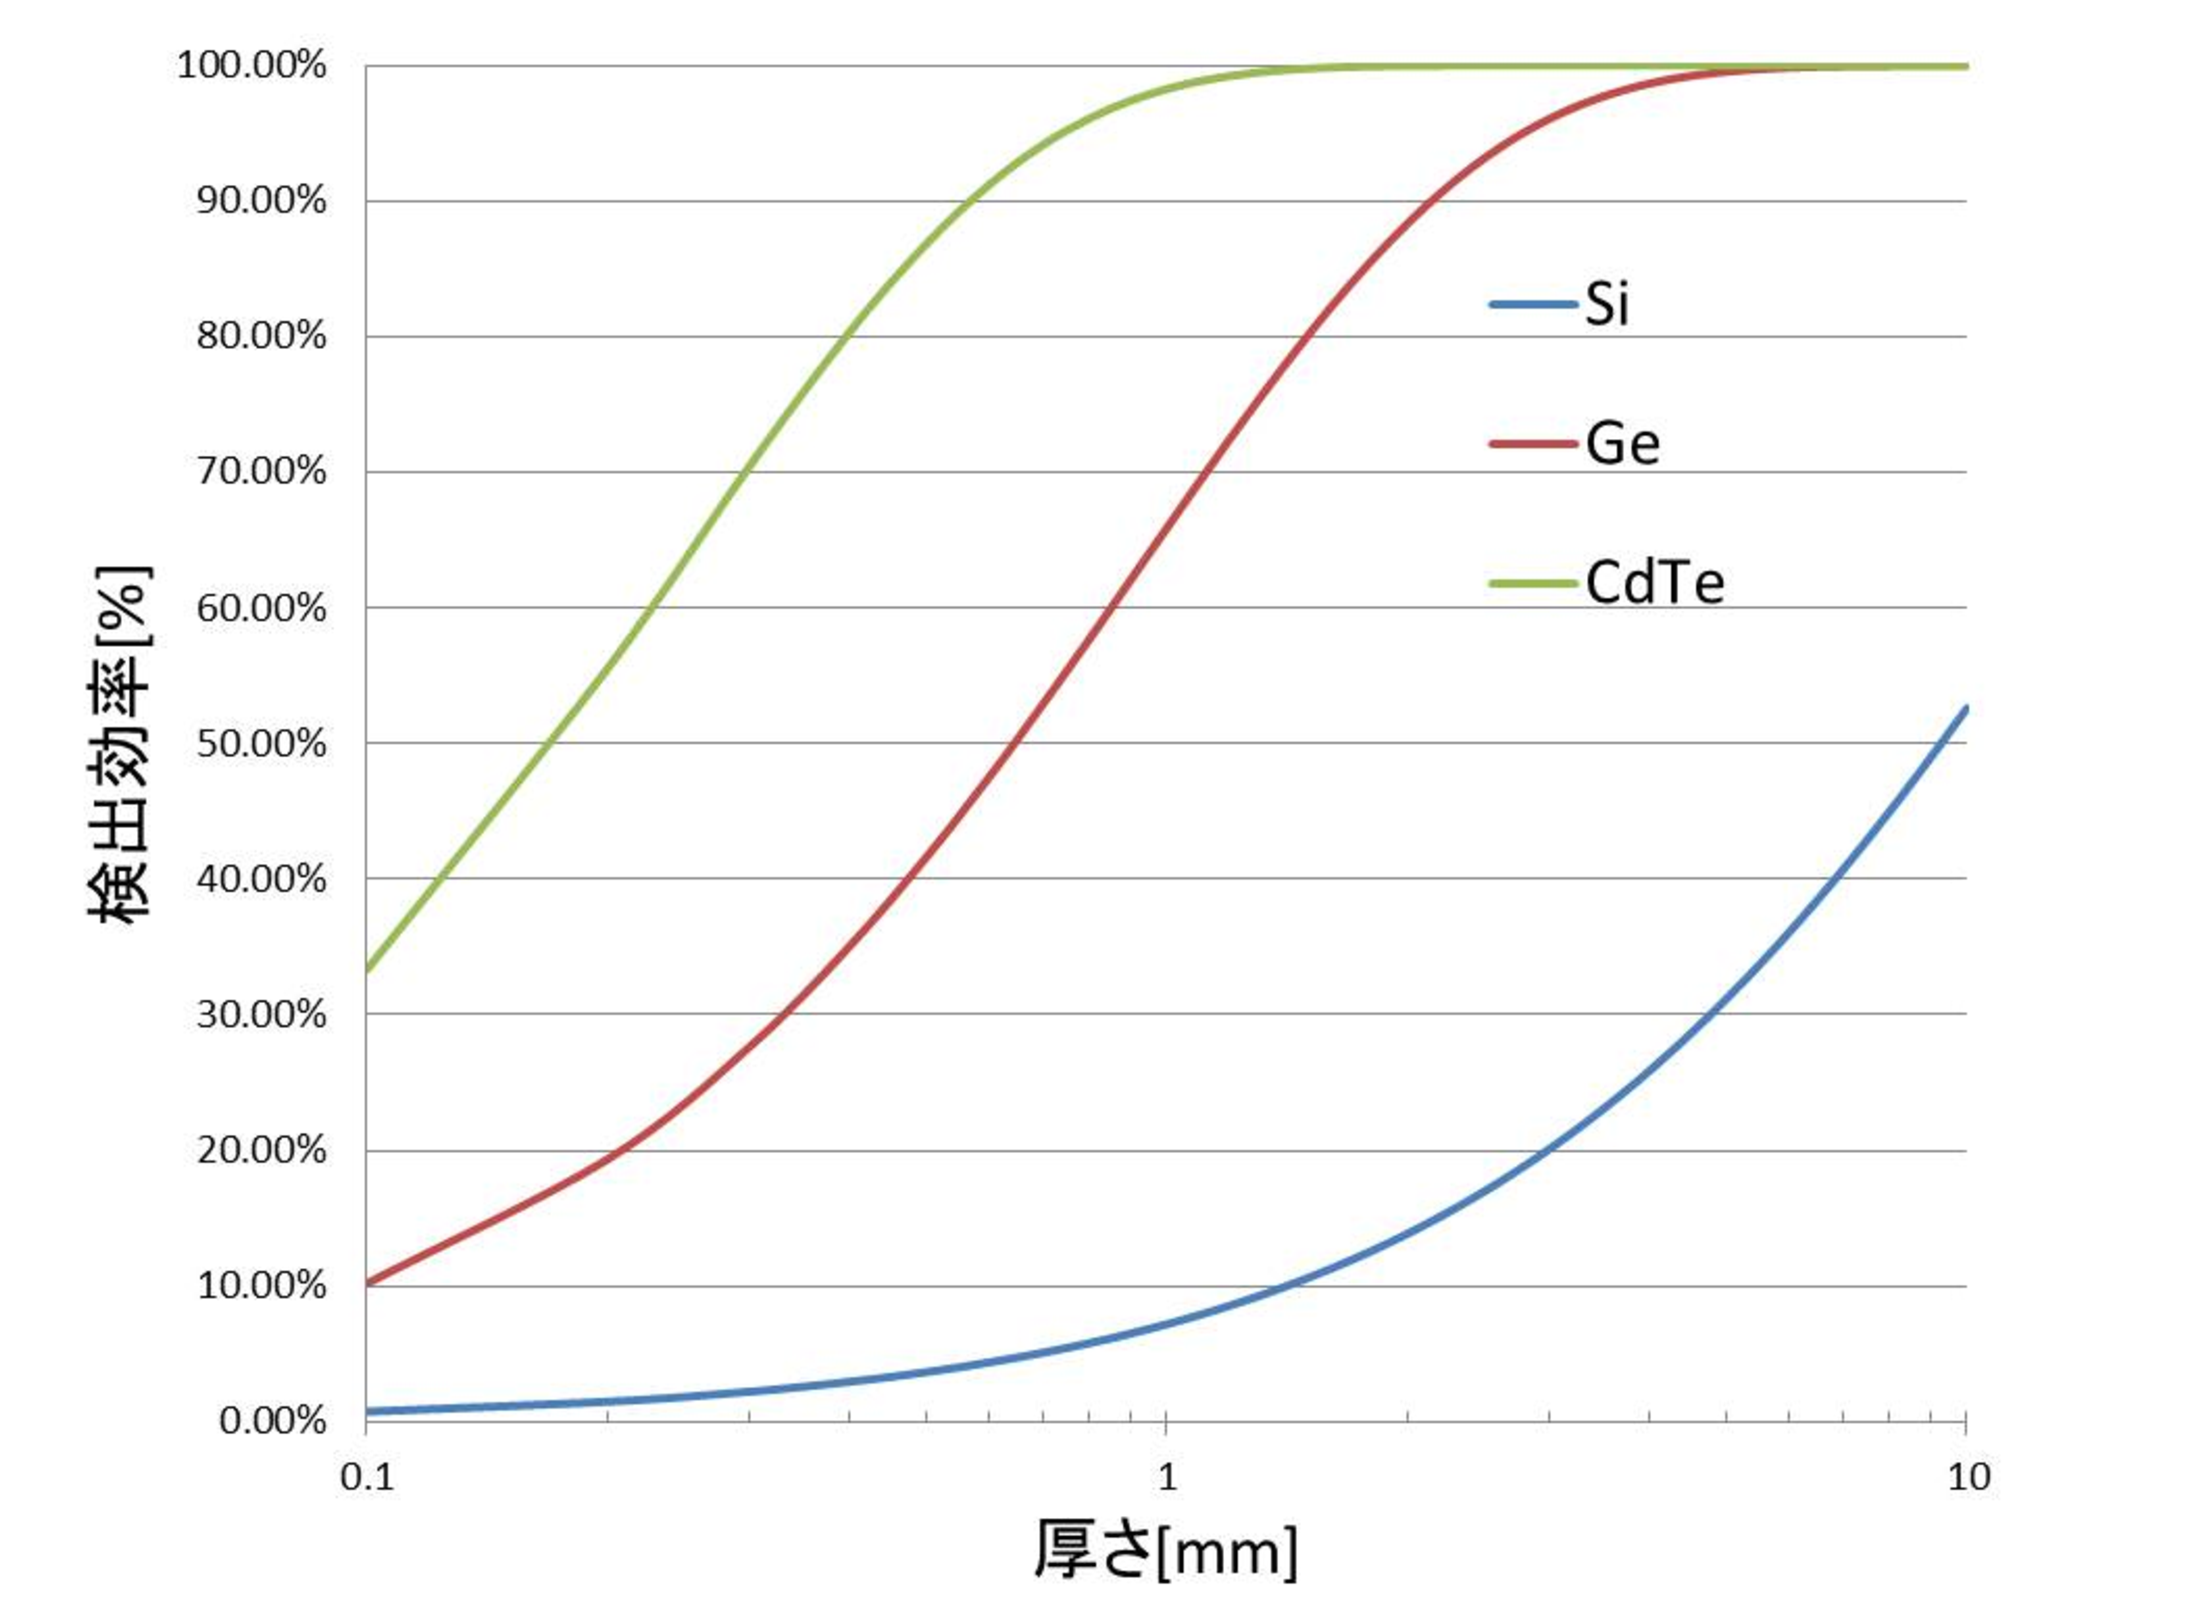
\includegraphics[width=8cm]{image/other/PDE_60.eps}
 \end{center}
 \end{minipage}
 \begin{minipage}{0.5\hsize}
 \begin{center}
 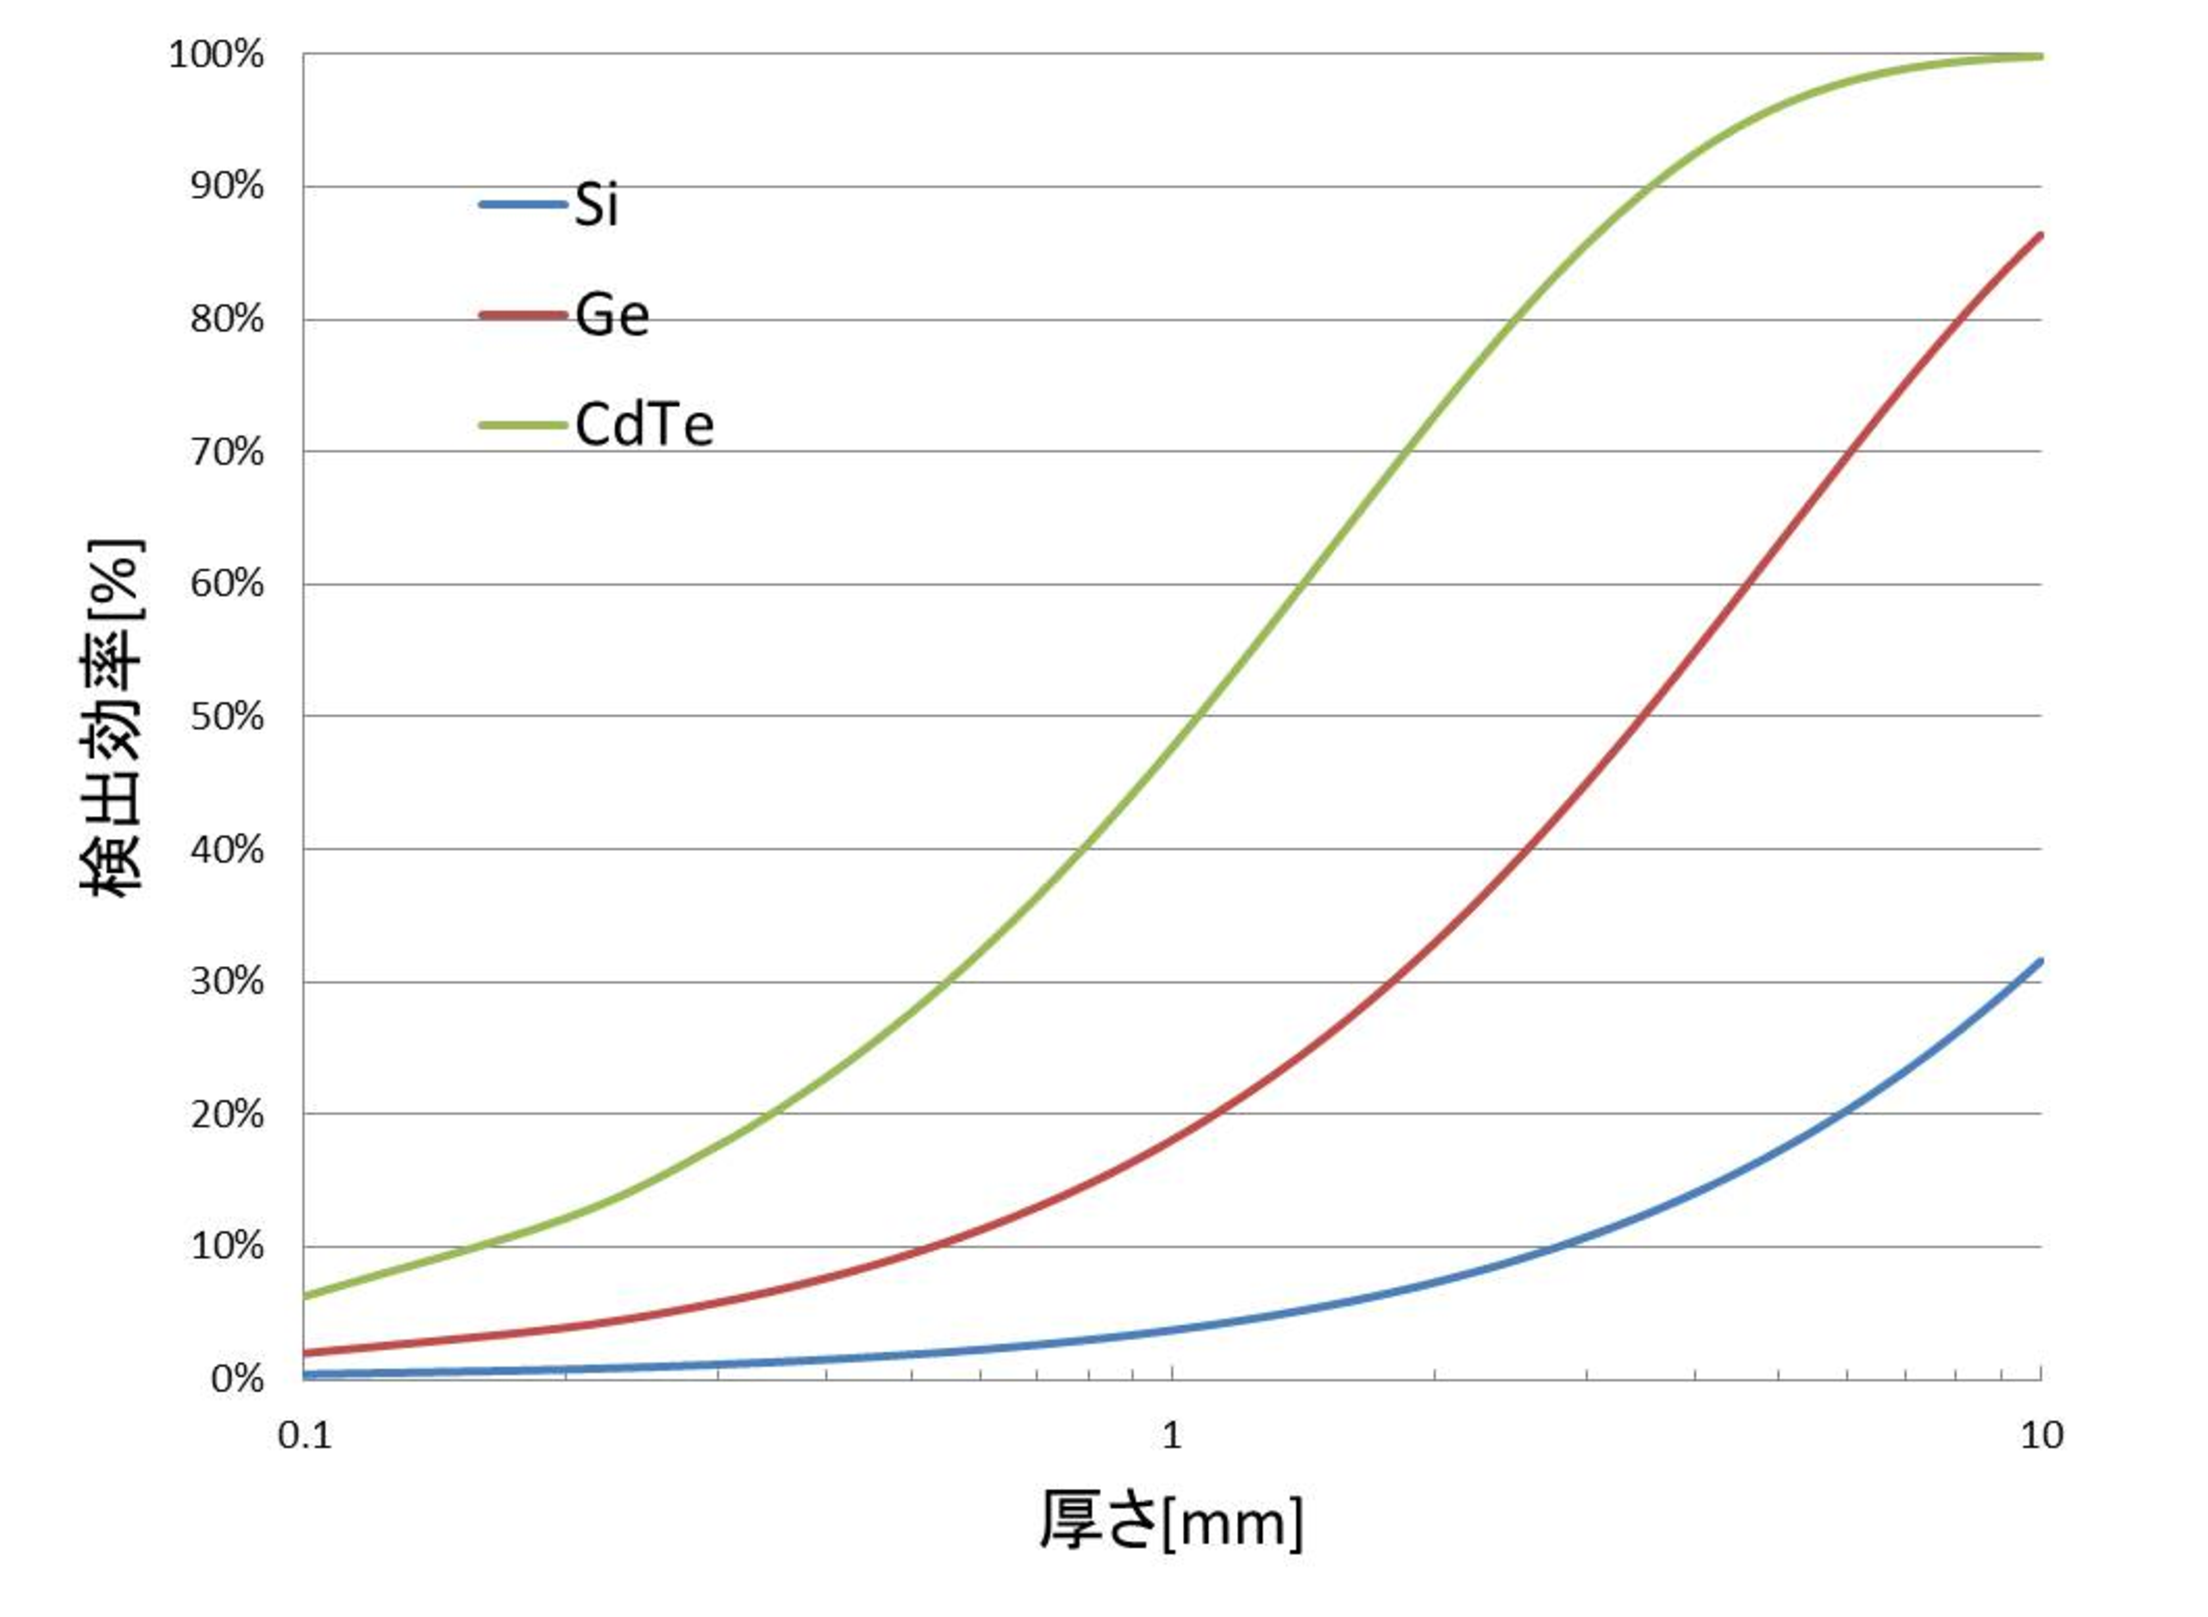
\includegraphics[width=8cm]{image/other/PDE_122.eps}
 \end{center}
  \end{minipage}
 \caption{Si,Ge,CdTeの60keV(左),120keV(右)に対する検出効率[NIST\cite{nist}より作成]}
 \label{fig:efficiency}
\end{figure}

\begin{figure}[H]
 \begin{center}
 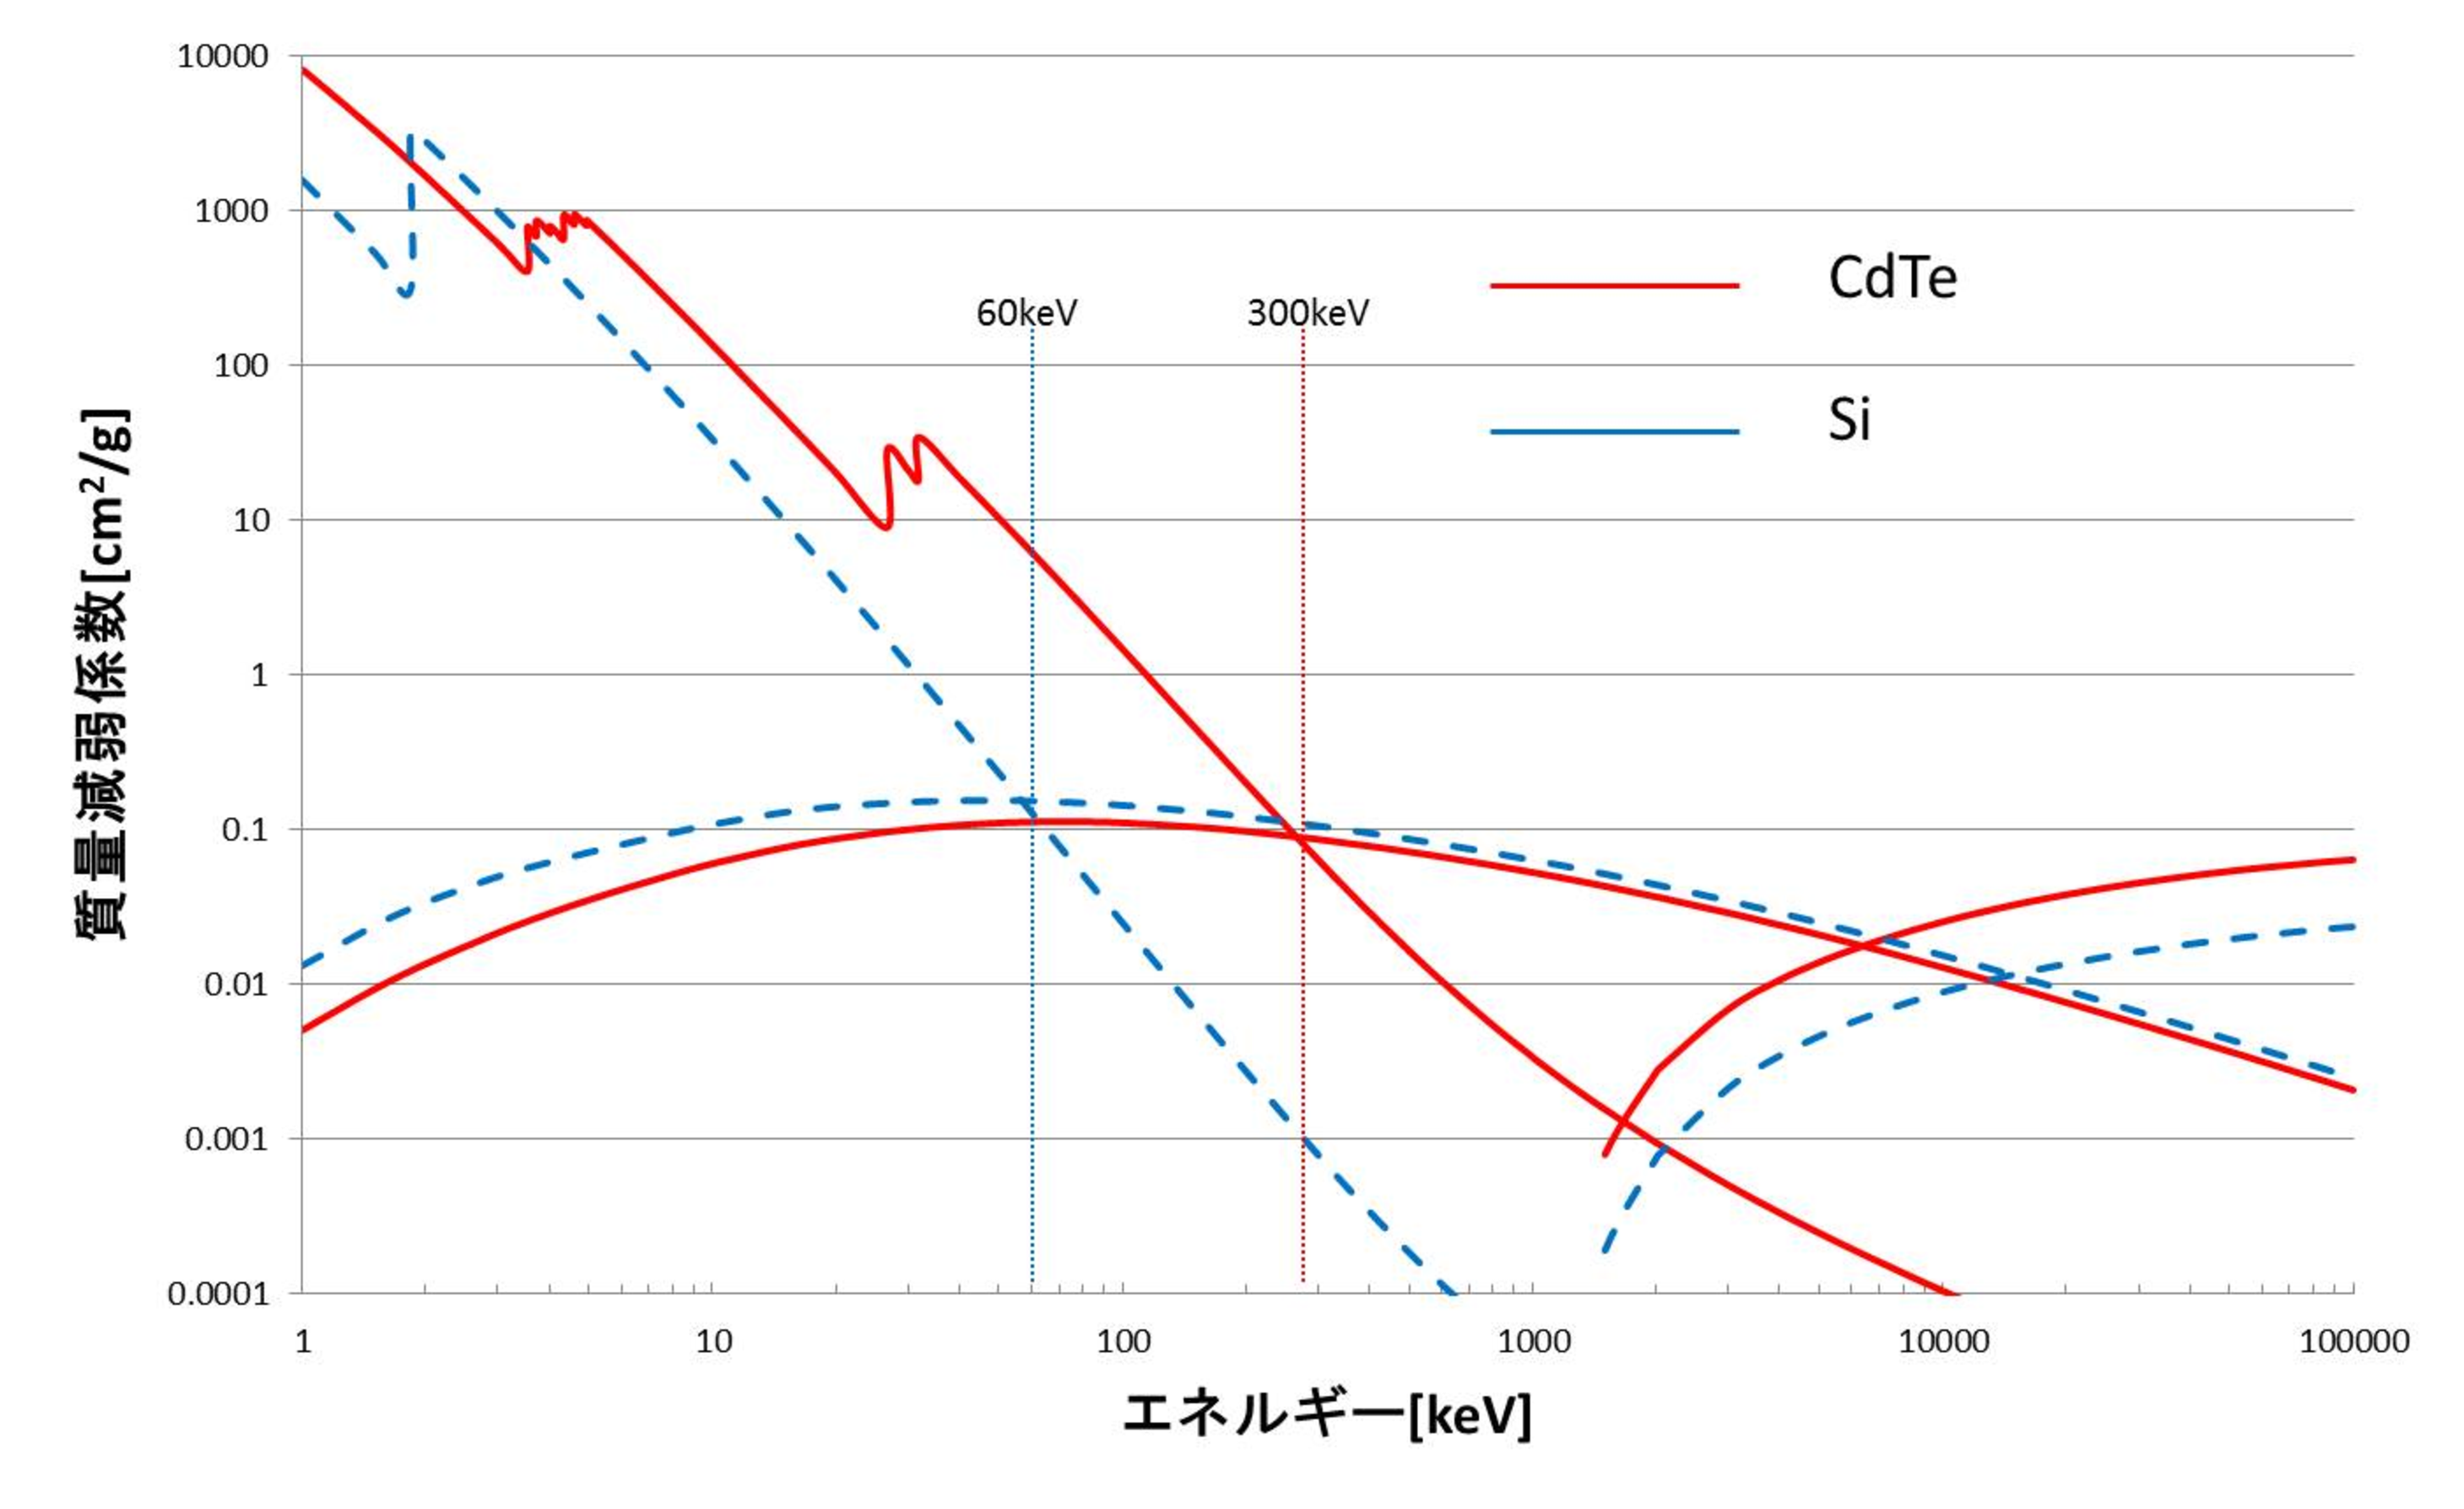
\includegraphics[width=10cm]{image/other/CdTe_Si.eps}
 \end{center}
 \caption{Si,Ge,CdTeに対する光子の光電吸収,コンプトン散乱,電子対生成による質量減弱係数[NIST\cite{nist}より作成]}
 \label{fig:liner_comp}
\end{figure}

\Fref{fig:efficiency}よりCdTeでは60keVのガンマ線に対しては1mmもあればほぼ100$\%$検出できるがSiでは1mmにおいては$7\%$程度しか検出できず,厚みを10mmにしてやっと約$50\%$検出できるようになる。また\Fref{fig:liner_comp}より高エネルギーにわたって光電効果が支配的であることが分かり,光電効果とコンプトン散乱の線源弱係数が等しくなるのはSiでは60keV,Geでは150keVであるのに対し,CdTeでは300keVで等しくなる。\\
\ \ 化合物半導体では,現存する最高の生成法を用いてもなお極く微量の不純物がな残存し,それらは電気的に活性なドーパントとして振舞う。例えば,アクセプタ準位を形成する不純物は材料を少しp型にし,その比抵抗を下げる。そこでバンドギャップ内に深いエネルギー準位を作る深いドナーを混ぜると,その補償作用により比抵抗を非常に大きくすることができる。同様の過程として,少しn型の材料の場合には深い準位を作る深いアクセプタを加える。こうした深いドナーやアクセプタは電荷キャリアの捕獲場所として働くため電荷キャリアの輸送を妨害する。この製法によりCdTeは非常に高い比抵抗($10^9\Omega$m)を持つようになる。

\section{CdTe半導体検出器の原理}

Siでは比抵抗が小さいので高電圧を印加した時のリーク電流が発生する。それを防ぐためpn接合によって比抵抗の高い空乏層を形成し,それを逆バイアスをかけて広げ有感層として用いたが,CdTeでは高い比抵抗を持つので結晶全体が有感層となり,結晶に電極(主に白金(Pt))をつけ単にバイアス電圧をかけることで検出器として用いることができる。この場合,CdTe検出器は固体電離箱として動作すると言える。

\section{CdTe半導体検出器のCT検出器利用における問題点\label{sec:CdTe}}

CdTeは結晶全体が有感層となり,多くの電子正孔対を発生するが,先述したように深いドナーやアクセプタによって電荷キャリアの輸送が妨害されるので,電荷キャリア特に正孔の移動度($\mu_h$)が小さく,寿命($\tau_h$)が短いということが問題である。\Tref{semi_chara}に示してあるが$\mu\tau$は電子,正孔においてSi,Geよりも小さく,CdTeの厚さが2mm程度の場合,電荷収集時間は$>500$nsとなる。そのためSi やGeでは生じた電荷を損なうことなく集めることができたが,CdTe では,途中で生じた電荷を損なってしまうのでCdTeを小型にせざるを得ない。そのためCTへの利用を考えた時にはピクセルサイズが小さくなり、読み出しチャンネル数が膨大になるという大きな課題を残すことになる。また低い$\mu\tau$によりパルス波高が電子正孔対の生成に位置によって異なり,スペクトルは低エネルギー側にテールを引いた形となり,エネルギー分解能はSi,Geよりも悪くなる。スペクトルのテールを低減するために高いバイアス電圧をかける必要がある。以下にその他の種々の問題点について述べる。

\begin{enumerate}
\item 信号を増幅するために前置増幅器が必要となるために長いテールを引いた信号となり、高計数においてはパイルアップしてしまう。
\item 放射線耐性が低く、経年劣化が激しい
\item 既存のCT装置を刷新する必要性がある
\item 高価である
\end{enumerate}
このようにCdTeを用いた検出器は早期における実用化・臨床応用においても多くの課題を残している。
%また,CdTe検出器は高ガンマ線束の下で電流モードで使われる。
%市販されているCdTe検出器は直径が1mmから1cmを少し超えるものまであり,厚さは2\UTF{FF5E}3mmかそれ以下に限られる。

%
\if0

\section{CdTe半導体を用いたピクセル検出器}
CdTeピクセル検出器とはX線やガンマ線の入った位置を検出し,撮像ができるようにしたものであり,その構造は\Fref{fig:pixel_CdTe}のように片側の電極を分割しピクセル化した構造になっている。それぞれのピクセル電極からの信号を一つ一つ別々のCSA,Shaping\ Ampで処理している。そのため読み出しチャンネル数は膨大になる。

\begin{figure}[H]
 \begin{center}
 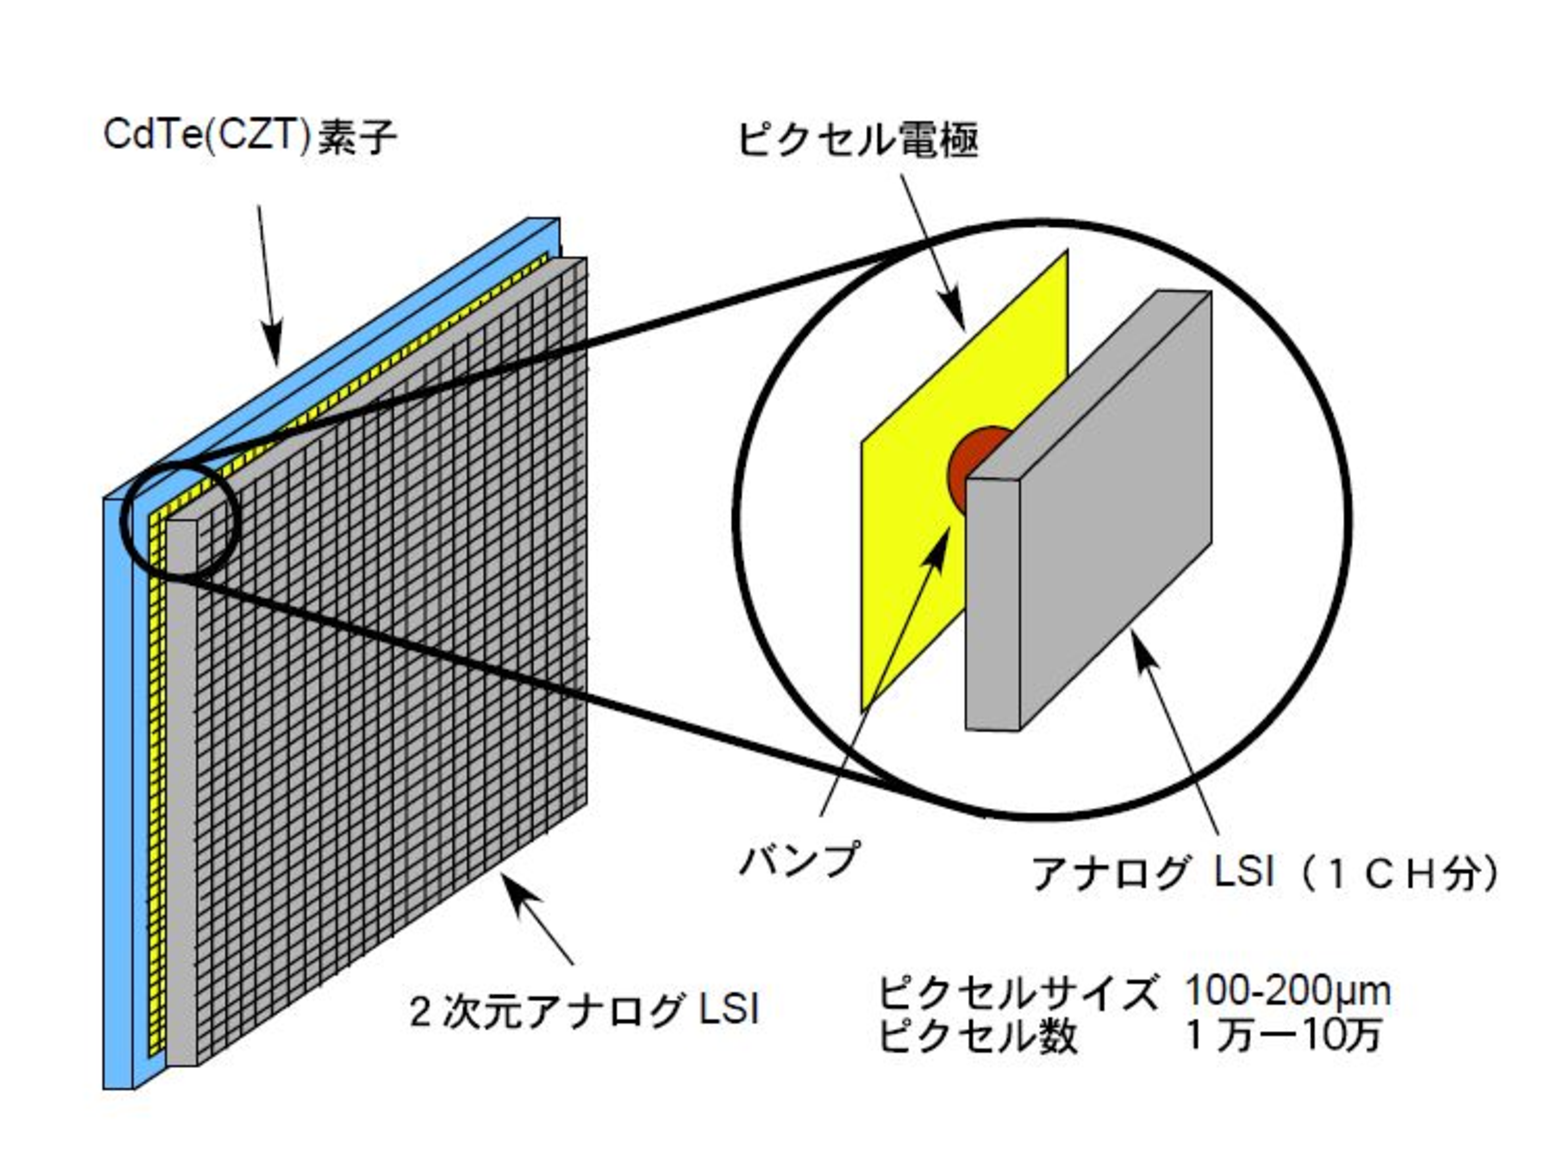
\includegraphics[width=10cm]{image/other/CdTe_pixel.eps}
 \end{center}
 \caption{CdTeピクセル検出器\cite{takahashi}}
 \label{fig:pixel_CdTe}
\end{figure}

%
\fi


